% !TeX document-id = {b1f9e40e-6197-4003-9b49-517a975e8757}
%===============================================================================
% LaTeX sjabloon voor de bachelorproef toegepaste informatica aan HOGENT
% Meer info op https://github.com/HoGentTIN/latex-hogent-report
%===============================================================================

\documentclass[dutch,dit,thesis]{hogentreport}

% TODO:
% - If necessary, replace the option `dit`' with your own department!
%   Valid entries are dbo, dbt, dgz, dit, dlo, dog, dsa, soa
% - If you write your thesis in English (remark: only possible after getting
%   explicit approval!), remove the option "dutch," or replace with "english".


\usepackage{lipsum} % For blind text, can be removed after adding actual content
%% Pictures to include in the text can be put in the graphics/ folder
\graphicspath{{graphics/}}

%% For source code highlighting, requires pygments to be installed
%% Compile with the -shell-escape flag!
\usepackage[section]{minted}
\usepackage{listings}
\definecolor{dkgreen}{rgb}{0,0.6,0}
\definecolor{gray}{rgb}{0.5,0.5,0.5}
\definecolor{mauve}{rgb}{0.58,0,0.82}

\lstset{frame=tb,
    language=Java,
    aboveskip=3mm,
    belowskip=3mm,
    showstringspaces=false,
    columns=flexible,
    basicstyle={\small\ttfamily},
    numbers=none,
    numberstyle=\tiny\color{gray},
    keywordstyle=\color{blue},
    commentstyle=\color{dkgreen},
    stringstyle=\color{mauve},
    breaklines=true,
    breakatwhitespace=true,
    tabsize=3
}
\usemintedstyle{solarized-light}
\definecolor{bg}{RGB}{253,246,227} %% Set the background color of the codeframe

%% Change this line to edit the line numbering style:
\renewcommand{\theFancyVerbLine}{\ttfamily\scriptsize\arabic{FancyVerbLine}}

%% Macro definition to load external java source files with \javacode{filename}:
\newmintedfile[javacode]{java}{
    bgcolor=bg,
    fontfamily=tt,
    linenos=true,
    numberblanklines=true,
    numbersep=5pt,
    gobble=0,
    framesep=2mm,
    funcnamehighlighting=true,
    tabsize=4,
    obeytabs=false,
    breaklines=true,
    mathescape=false
    samepage=false,
    showspaces=false,
    showtabs =false,
    texcl=false,
}

% Other packages not already included can be imported here

%%---------- Document metadata -------------------------------------------------
% TODO: Replace this with your own information
\author{Kobe Dehandschutter}
\supervisor{S. Lievens}
\cosupervisor{M. Verstraeten}
\title%
    {De mogelijkheden voor data-extractie in ongestructureerde masterdata op basis van clustering: een vergelijkende studie}
\academicyear{\advance\year by -1 \the\year--\advance\year by 1 \the\year}
\examperiod{1}
\degreesought{\IfLanguageName{dutch}{Professionele bachelor in de toegepaste informatica}{Bachelor of applied computer science}}
\partialthesis{false} %% To display 'in partial fulfilment'
%\institution{Internshipcompany BVBA.}

%% Add global exceptions to the hyphenation here
\hyphenation{back-slash}

%% The bibliography (style and settings are  found in hogentthesis.cls)
\addbibresource{bachproef.bib}            %% Bibliography file
\addbibresource{../voorstel/voorstel.bib} %% Bibliography research proposal
\defbibheading{bibempty}{}

%% Prevent empty pages for right-handed chapter starts in twoside mode
\renewcommand{\cleardoublepage}{\clearpage}

\renewcommand{\arraystretch}{1.2}

%% Content starts here.
% !TeX TXS-program:compile = txs:///pdflatex/[--shell-escape]s
\begin{document}

%---------- Front matter -------------------------------------------------------

\frontmatter

\hypersetup{pageanchor=false} %% Disable page numbering references
%% Render a Dutch outer title page if the main language is English
\IfLanguageName{english}{%
    %% If necessary, information can be changed here
    \degreesought{Professionele Bachelor toegepaste informatica}%
    \begin{otherlanguage}{dutch}%
       \maketitle%
    \end{otherlanguage}%
}{}

%% Generates title page content
\maketitle
\hypersetup{pageanchor=true}

%%=============================================================================
%% Voorwoord
%%=============================================================================

\chapter*{\IfLanguageName{dutch}{Woord vooraf}{Preface}}%
\label{ch:voorwoord}

%% TODO:
%% Het voorwoord is het enige deel van de bachelorproef waar je vanuit je
%% eigen standpunt (``ik-vorm'') mag schrijven. Je kan hier bv. motiveren
%% waarom jij het onderwerp wil bespreken.
%% Vergeet ook niet te bedanken wie je geholpen/gesteund/... heeft

\lipsum[1-2]
%%=============================================================================
%% Samenvatting
%%=============================================================================

% TODO: De "abstract" of samenvatting is een kernachtige (~ 1 blz. voor een
% thesis) synthese van het document.
%
% Een goede abstract biedt een kernachtig antwoord op volgende vragen:
%
% 1. Waarover gaat de bachelorproef?
% 2. Waarom heb je er over geschreven?
% 3. Hoe heb je het onderzoek uitgevoerd?
% 4. Wat waren de resultaten? Wat blijkt uit je onderzoek?
% 5. Wat betekenen je resultaten? Wat is de relevantie voor het werkveld?
%
% Daarom bestaat een abstract uit volgende componenten:
%
% - inleiding + kaderen thema
% - probleemstelling
% - (centrale) onderzoeksvraag
% - onderzoeksdoelstelling
% - methodologie
% - resultaten (beperk tot de belangrijkste, relevant voor de onderzoeksvraag)
% - conclusies, aanbevelingen, beperkingen
%
% LET OP! Een samenvatting is GEEN voorwoord!



%%---------- Samenvatting -----------------------------------------------------
% De samenvatting in de hoofdtaal van het document

\chapter*{\IfLanguageName{dutch}{Samenvatting}{Abstract}}

Het beheren van ongestructureerde masterdata is een probleem waar veel bedrijven mee kampen. Het is heel lastig om structuur te brengen in zulke tabellen. In dit onderzoek worden verschillende manieren vergeleken om deze data te clusteren zodat gelijkaardige data gegroepeerd wordt. Aan de hand daarvan kunnen bedrijven de beste methode vinden om de datakwaliteit van hun masterdata te verbeteren.
\\\indent
Ongestructureerde masterdata bestaat in alle vormen en maten, daarom wordt in dit onderzoek gebruik gemaakt van drie verschillende datasets. De eerste bevat productinformatie die bestaat uit een paar woorden, codes en afmetingen. De tweede set bevat informatie over wijnen in de vorm van lange zinnen. De derde bevat opnieuw productinformatie, maar deze keer zonder codes of afmetingen, enkel bestaande woorden.
\\\indent
Wanneer alle mogelijke clustermethodes besproken zijn, worden de drie meest geschikte methodes uitgewerkt, namelijk K-means, dbscan en Hiërarchisch clusteren. De algoritmes K-means en dbscan verwachten de data echter in getallen in plaats van in woorden. Ook hiervoor worden verschillende manieren gezocht en de twee meest geschikte manieren hiervoor worden uitgewerkt, namelijk tf-idf en word2vec.
\\\indent
Hiërarchisch clusteren verwacht de data niet in getallen zoals de andere methodes, maar dit algoritme verwacht een matrix met alle afstanden tussen iedere waarde van de dataset. Om dit te bereiken zijn er opnieuw een aantal mogelijkheden. In dit onderzoek wordt de Levenshtein distance gebruikt.
\\\indent
Uiteindelijk zijn er vijf verschillende combinaties die uitgewerkt worden:
\begin{enumerate}
    \item Tf-idf met K-means.
    \item Tf-idf met dbscan.
    \item Levenshtein distance met hiërarchisch clusteren.
    \item Word2vec met K-means.
    \item Word2vec met dbscan.
\end{enumerate}
\\\indent
Het uitwerken van de algoritmes gebeurt in Python, aangezien er in Python heel wat bibliotheken bestaan die helpen bij het opstellen van deze algoritmes. Alle vijf de combinaties worden uitgevoerd met alle drie de datasets en de resultaten worden vergeleken op basis van het aantal clusters, de grootste cluster, een eventuele vuilniscluster die restwaarden bevat en het Silhoutte gemiddelde. Dit Silhoutte gemiddelde is een manier om de accuraatheid van een ongesuperviseerd clusteralgoritme te berekenen.
\\\indent
Uit de resultaten van de vergelijkende studie komt tf-idf in combinatie met K-means naar voren als de beste manier om ongestructureerde masterdata te clusteren. Dit is echter enkel het geval voor de twee datasets met productdata. Voor de dataset met de lange zinnen is geen enkele methode geslaagd in het succesvol clusteren van deze data. Hopelijk kan ik aan de hand van dit onderzoek iemand op weg helpen om een geschikte manier hiervoor te vinden.
\\\indent





%---------- Inhoud, lijst figuren, ... -----------------------------------------

\tableofcontents

% In a list of figures, the complete caption will be included. To prevent this,
% ALWAYS add a short description in the caption!
%
%  \caption[short description]{elaborate description}
%
% If you do, only the short description will be used in the list of figures

\listoffigures

% If you included tables and/or source code listings, uncomment the appropriate
% lines.
%\listoftables
%\listoflistings

% Als je een lijst van afkortingen of termen wil toevoegen, dan hoort die
% hier thuis. Gebruik bijvoorbeeld de ``glossaries'' package.
% https://www.overleaf.com/learn/latex/Glossaries

%---------- Kern ---------------------------------------------------------------

\mainmatter{}

% De eerste hoofdstukken van een bachelorproef zijn meestal een inleiding op
% het onderwerp, literatuurstudie en verantwoording methodologie.
% Aarzel niet om een meer beschrijvende titel aan deze hoofdstukken te geven of
% om bijvoorbeeld de inleiding en/of stand van zaken over meerdere hoofdstukken
% te verspreiden!

%%=============================================================================
%% Inleiding
%%=============================================================================

\chapter{\IfLanguageName{dutch}{Inleiding}{Introduction}}%
\label{ch:inleiding}

De inleiding moet de lezer net genoeg informatie verschaffen om het onderwerp te begrijpen en in te zien waarom de onderzoeksvraag de moeite waard is om te onderzoeken. In de inleiding ga je literatuurverwijzingen beperken, zodat de tekst vlot leesbaar blijft. Je kan de inleiding verder onderverdelen in secties als dit de tekst verduidelijkt. Zaken die aan bod kunnen komen in de inleiding~\autocite{Pollefliet2011}:

\begin{itemize}
  \item context, achtergrond
  \item afbakenen van het onderwerp
  \item verantwoording van het onderwerp, methodologie
  \item probleemstelling
  \item onderzoeksdoelstelling
  \item onderzoeksvraag
  \item \ldots
\end{itemize}

\section{\IfLanguageName{dutch}{Probleemstelling}{Problem Statement}}%
\label{sec:probleemstelling}

Uit je probleemstelling moet duidelijk zijn dat je onderzoek een meerwaarde heeft voor een concrete doelgroep. De doelgroep moet goed gedefinieerd en afgelijnd zijn. Doelgroepen als ``bedrijven,'' ``KMO's'', systeembeheerders, enz.~zijn nog te vaag. Als je een lijstje kan maken van de personen/organisaties die een meerwaarde zullen vinden in deze bachelorproef (dit is eigenlijk je steekproefkader), dan is dat een indicatie dat de doelgroep goed gedefinieerd is. Dit kan een enkel bedrijf zijn of zelfs één persoon (je co-promotor/opdrachtgever).

\section{\IfLanguageName{dutch}{Onderzoeksvraag}{Research question}}%
\label{sec:onderzoeksvraag}

Wees zo concreet mogelijk bij het formuleren van je onderzoeksvraag. Een onderzoeksvraag is trouwens iets waar nog niemand op dit moment een antwoord heeft (voor zover je kan nagaan). Het opzoeken van bestaande informatie (bv. ``welke tools bestaan er voor deze toepassing?'') is dus geen onderzoeksvraag. Je kan de onderzoeksvraag verder specifiëren in deelvragen. Bv.~als je onderzoek gaat over performantiemetingen, dan 

\section{\IfLanguageName{dutch}{Onderzoeksdoelstelling}{Research objective}}%
\label{sec:onderzoeksdoelstelling}

Wat is het beoogde resultaat van je bachelorproef? Wat zijn de criteria voor succes? Beschrijf die zo concreet mogelijk. Gaat het bv.\ om een proof-of-concept, een prototype, een verslag met aanbevelingen, een vergelijkende studie, enz.

\section{\IfLanguageName{dutch}{Opzet van deze bachelorproef}{Structure of this bachelor thesis}}%
\label{sec:opzet-bachelorproef}

% Het is gebruikelijk aan het einde van de inleiding een overzicht te
% geven van de opbouw van de rest van de tekst. Deze sectie bevat al een aanzet
% die je kan aanvullen/aanpassen in functie van je eigen tekst.

De rest van deze bachelorproef is als volgt opgebouwd:

In Hoofdstuk~\ref{ch:stand-van-zaken} wordt een overzicht gegeven van de stand van zaken binnen het onderzoeksdomein, op basis van een literatuurstudie.

In Hoofdstuk~\ref{ch:methodologie} wordt de methodologie toegelicht en worden de gebruikte onderzoekstechnieken besproken om een antwoord te kunnen formuleren op de onderzoeksvragen.

% TODO: Vul hier aan voor je eigen hoofstukken, één of twee zinnen per hoofdstuk

In Hoofdstuk~\ref{ch:conclusie}, tenslotte, wordt de conclusie gegeven en een antwoord geformuleerd op de onderzoeksvragen. Daarbij wordt ook een aanzet gegeven voor toekomstig onderzoek binnen dit domein.
\chapter{\IfLanguageName{dutch}{Stand van zaken}{State of the art}}%
\label{ch:stand-van-zaken}

% Tip: Begin elk hoofdstuk met een paragraaf inleiding die beschrijft hoe
% dit hoofdstuk past binnen het geheel van de bachelorproef. Geef in het
% bijzonder aan wat de link is met het vorige en volgende hoofdstuk.

% Pas na deze inleidende paragraaf komt de eerste sectiehoofding.

Dit hoofdstuk bevat je literatuurstudie. De inhoud gaat verder op de inleiding, maar zal het onderwerp van de bachelorproef *diepgaand* uitspitten. De bedoeling is dat de lezer na lezing van dit hoofdstuk helemaal op de hoogte is van de huidige stand van zaken (state-of-the-art) in het onderzoeksdomein. Iemand die niet vertrouwd is met het onderwerp, weet nu voldoende om de rest van het verhaal te kunnen volgen, zonder dat die er nog andere informatie moet over opzoeken \autocite{Pollefliet2011}.

Je verwijst bij elke bewering die je doet, vakterm die je introduceert, enz.\ naar je bronnen. In \LaTeX{} kan dat met het commando \texttt{$\backslash${textcite\{\}}} of \texttt{$\backslash${autocite\{\}}}. Als argument van het commando geef je de ``sleutel'' van een ``record'' in een bibliografische databank in het Bib\LaTeX{}-formaat (een tekstbestand). Als je expliciet naar de auteur verwijst in de zin, gebruik je \texttt{$\backslash${}textcite\{\}}.
Soms wil je de auteur niet expliciet vernoemen, dan gebruik je \texttt{$\backslash${}autocite\{\}}. In de volgende paragraaf een voorbeeld van elk.

\textcite{Knuth1998} schreef een van de standaardwerken over sorteer- en zoekalgoritmen. Experten zijn het erover eens dat cloud computing een interessante opportuniteit vormen, zowel voor gebruikers als voor dienstverleners op vlak van informatietechnologie~\autocite{Creeger2009}.

\lipsum[7-20]

%%=============================================================================
%% Methodologie
%%=============================================================================

\chapter{\IfLanguageName{dutch}{Methodologie}{Methodology}}%

\label{ch:methodologie}

%% TODO: Hoe ben je te werk gegaan? Verdeel je onderzoek in grote fasen, en
%% licht in elke fase toe welke stappen je gevolgd hebt. Verantwoord waarom je
%% op deze manier te werk gegaan bent. Je moet kunnen aantonen dat je de best
%% mogelijke manier toegepast hebt om een antwoord te vinden op de
%% onderzoeksvraag.



Zoals vele onderzoeken wordt hier ook begonnen met een requirements analyse. Op die manier is het duidelijk welke eigenschappen van de algoritmes belangrijk zijn voor deze onderzoeksvraag.



\section{Requirements analyse}

\begin{itemize}
    \item1. Must have: Gemiddelde aantal waarden per cluster > 5
    \item2. Should have: Grootste cluster bevat minder dan 5\% van het aantal waarden
    \item3. Could have: Silhoutte average > 0.25
    \item4. Won't have: Een vuilniscluster die meer dan 20\% van alle waarden bevat.
\end{itemize}
\\\indent
Het is moeilijk een ideale voorspelling te doen voor het gemiddelde aantal waarden per cluster. In het geval dat de data perfect in twee clusters kan verdeeld worden, zal het gemiddelde heel hoog liggen terwijl de clusters ook succesvol zijn. Er is dus geen maximum op dit gemiddelde. Een minimum is echter wel verplicht. Wanneer dit gemiddelde lager dan vijf zou liggen, betekent dat dat de clusters veel te klein zijn om als succesvol beschouwt te worden.
\\\indent
Als tweede zou de grootste cluster best minder dan 5\% van alle waarden bevatten. Het is een should have, want er kunnen op zich gevallen zijn waar meer dan vijf procent wel degelijk in dezelfde cluster hoort, maar in de meeste gevallen en in de datasets die in dit onderzoek gebruikt worden, is dit niet het geval.
\\\indent
Als derde is er de Silhoutte average. Dit is een score tussen -1 en 1 en deze wordt berekend door voor iedere waarde te kijken of deze in de juiste cluster zit, of dichter aanleunt bij een andere cluster. Hoe hoger het gemiddelde, hoe beter de clusters. Dit is een could have, want dit kan soms bedrieglijk overkomen. Wanneer er bijvoorbeeld maar één cluster is en alle waarden zitten in diezelfde cluster, dan is dit gemiddelde 1 aangezien geen elke waarde beter in een andere cluster thuishoort, want er zijn geen andere clusters.
\\\indent
Als vierde is er ook een won't have, in de meeste gevallen zal er een vuilniscluster aangemaakt worden waar waarden in belanden die nergens anders bijpassen. Het is echter zeker niet de bedoeling dat deze cluster te groot wordt, want dan worden de resultaten niet meer nuttig. De maximumgrootte voor deze vuilniscluster wordt dus op 20\% gelegd. Als er dus 1000 waarden zijn, mogen er maximum 200 zijn die niet tot een goede clusters behoren.
\\\indent



\section{Short-list}
Uit alle algoritmes die besproken geweest zijn in de literatuurstudie, zijn er vijf finale combinaties overgebleven die onderzocht en vergeleken zullen worden. Hiërarchisch clusteren heeft een methode nodig om de afstand tussen twee waarden te berekenen. Dit wordt gecombineerd met de levenshtein distance, wat een goede en eenvoudige manier is om dit te bepalen. De twee andere clustermethoden, K-means en dbscan hebben een methode nodig die de tekst kan omzetten in nummers. Hiervoor zijn er twee geschikte methoden gevonden, die op een heel verschillende manier te werk gaan, namelijk tf-idf en word2vec. De vijf combinaties zijn als volgt:
\begin{itemize}
    \item1. Tf-idf en K-means
    \item2. Tf-idf en dbscan
    \item3. Word2vec en K-means
    \item4. Word2vec en dbScan
    \item5. Levenshtein en hiërarchical clustering
\end{itemize}

\section{Gebruikte data}
Dit onderzoek maakt gebruik van drie datasets met ongestructureerde data. De eerste dataset komt rechtstreeks uit de praktijk, heeft 4146 waarden en bevat productdata. Een voorbeeld van een waarde uit deze dataset is: '100mm Knauf Rocksilk Flexi Slab (4.32m²)'. Bij veel waarden in deze set zijn ook de afmetingen vermeld. Deze informatie is echter niet interessant, aangezien stukken hout van 100mm en van 140mm tot dezelfde cluster behoren. Om een beter resultaat te verkrijgen worden alle getallen in deze set op 0 gezet. Zo blijft het duidelijk dat de data een afmeting bevat, maar de grootte van die afmeting is irrelevant.
\\\indent
De tweede dataset bevat 4000 waardes omtrent wijn en is afkomstig van `Kaggle` \autocite{Iv2018}. Een voorbeeld van een waarde uit deze set: 'The variety is unmistakable, with notes of dried herb, dark cherry and espresso. The jammy fruit flavors are rich, with lightly grainy tannins and coffee notes on the finish. It shows a fine sense of balance.'. De waardes uit deze set zijn duidelijk een stuk langer en bevatten geen afkortingen of getallen.
\\\indent
De derde dataset is gevonden op 'UCI' en bevat 5000 waarden \autocite{Chen2012}. Deze set bevat opnieuw productdata, maar ook deze heeft geen getallen of afkortingen. Een voorbeeld van een waarde uit deze set: 'GREY HEART HOT WATER BOTTLE'.
\\\indent
\begin{lstlisting}
    df_original = pd.read_csv("data.csv", delimiter=';')
    chosen_column = "Material Description EN"

    df_original[chosen_column] = df_original[chosen_column].str.replace('[0-9]', '0', regex=True)
\end{lstlisting}
\\\indent
Om deze datasets te kunnen gebruiken in Python, wordt gebruik gemaakt van pandas. Pandas is een Python bibliotheek die heel veel kan, onder andere csv bestanden inlezen. De delimiter die wordt meegegeven is de aanduiding waar een waarde in de kolom eindigt en de volgende waarde begint. De chosen\_column waarde is de naam van de kolom die wordt gebruikt, in dit geval is dit de kolom met materiaal beschrijvingen. Door 'df\_original[chosen\_column]' op te roepen, wordt de juiste kolom uit de dataset verkregen. Tot slot worden, zoals hiervoor besproken, alle getallen tussen 0 en 9 vervangen door een 0.



\section{Opmaken algoritmes in Python}


\subsection{tf-idf}
Nu de short-list is opgesteld en de data ingelezen is, is de volgende stap het uitwerken van de algoritmen in Python. Er wordt begonnen met tf-idf. De TfidfVectorizer wordt geïmporteerd van sklearn. Tf-idf wordt uitgevoerd met n-grammen, maar deze kunnen op basis van karakters of volledige woorden zijn. De variabele chosen\_ngrams bepaalt dit: als de waarde 'char' is, zijn het karakters, is de waarde 'word' dan is het met woorden.
\\\indent
\begin{lstlisting}
    from sklearn.feature_extraction.text import TfidfVectorizer

    chosen_ngrams = "char"
    chosen_ngram_range = (2, 4)
    tfidf_vectorizer=TfidfVectorizer(use_idf=True, analyzer = chosen_ngrams, ngram_range=chosen_ngram_range)
    tfidf_vectorizer_vectors = tfidf_vectorizer.fit_transform(df_original[chosen_column].to_list())
\end{lstlisting}
\\\indent
 De volgende variabele bepaalt de n-gram range, in dit geval wordt gewerkt met 2-grammen, 3-grammen en 4-grammen. Vervolgens wordt een vectorizer aangemaakt aan de hand van deze twee variabelen. Deze vectorizer wordt gebruikt op de kolom met data zodat tfidf\_vectorizer\_vectors een lijst met alle vectoren van de waarden bevat.




\subsection{K-means}
Om K-means te kunnen gebruiken, moet het aantal clusters op voorhand beslist worden. De manier die hiervoor gebruikt wordt in dit onderzoek, wordt in het volgende hoofdstuk genaamd 'Canopy clustering' uitgelegd. Voorlopig wordt met een waarde van 20 gewerkt.
\\\indent
De KMeans() functie wordt geïmporteerd van sklearn, het aantal clusters en de vectoren van tf-idf worden hier als parameter meegegeven. Vervolgens wordt de pandas bibliotheek opnieuw gebruikt om een nieuwe dataframe aan te maken die twee kolommen bevat. De eerste kolom bevat de labels die de KMeans functie teruggegeven heeft, de tweede kolom bevat de productbeschrijvingen. Dit ziet er als volgt uit:

\\\indent 5 , 000mm F/F Cladding Roll 0000x0000
\\\indent18 , 000mm Kingspan TP00 PIR (0.00m²)
\\\indent18 , 000mm Kingspan TR00 PIR (0.00m²)

De Cladding Roll zit in cluster nummer vijf, de twee kingspannen, waarbij de afmetingen op 0 geplaatst zijn om identieke waardes to bekomen, zitten in cluster nummer achttien.

\begin{lstlisting}
kmeans = KMeans(20).fit(tfidf_vectorizer_vectors)
df_clustered = pd.DataFrame({'cluster': kmeans.labels_, 'value': df_original[chosen_column].to_list()})
\end{lstlisting}

\\\indent



\subsection{Canopy clustering}
Om K-means te kunnen gebruiken, moet het aantal clusters op voorhand beslist worden. In dit onderzoek wordt dit aantal bepaald door canopy clustering. Zoals besproken in de literatuurstudie is deze manier van clusteren niet zo accuraat, maar berekent deze wel zelf het aantal clusters. Hieronder is de functie te zien die gebruikt wordt om het aantal clusters te berekenen. Deze functie heeft vier parameters:
\begin{enumerate}
    \item X: De dataset in de vorm van een lijst met vectoren.
    \item T1: Loose distance.
    \item T2: Tight distance.
    \item Distance metric: De manier om de afstand te berekenen, deze staat standaard op de euclidean distance.
\end{enumerate}
\\\indent
\begin{lstlisting}
    def canopy(X, T1, T2, distance_metric='euclidean'):
    canopies = dict()
    X1_dist = pairwise_distances(X, metric=distance_metric)
    canopy_points = set(range(X.shape[0]))
    while canopy_points:
    point = canopy_points.pop()
    i = len(canopies)
    canopies[i] = {"c":point, "points": list(np.where(X1_dist[point] < T1)[0])}
    canopy_points = canopy_points.difference(set(np.where(X1_dist[point] < T2)[0]))
    return len(canopies)
\end{lstlisting}
\\\indent
De functie begint met het aanmaken van een lege dictionary om hier uiteindelijk alle clusters in op te nemen. Vervolgens wordt de pairwise\_distances functie gebruikt van sklearn. Deze geeft een matrix terug met alle afstanden tussen alle waarden van de array, zodat geldt dat X1\_dist[i,j] de afstand is tussen de waarden i en j uit de originele array van vectoren. Hierna maakt de functie een set aan die alle indices van de array van vectoren bevat. Zolang er waardes in de set zitten, worden volgende acties doorlopen:
\begin{itemize}
    \item De laatste index wordt verwijderd, dit wordt het centerpunt van de nieuwe cluster.
    \item Er wordt een nieuwe cluster aangemaakt in de dictonairy.
    \item Aan die nieuwe cluster worden alle resterende waarden toegevoegd waarvan hun afstand tot het centerpunt kleiner is dan T1.
    \item Alle indices waarvoor deze afstand ook kleiner is dan T2 worden uit de canopy\_points set verwijderd.
\end{itemize}
Van zodra alle waardes in de set verwijderd zijn, wordt het aantal clusters teruggegeven.
\\\indent
Aangezien enkel het aantal clusters belangrijk is en niet wat er precies in de cluster zit, is T1 in deze situatie irrelevant. T2 is wel belangrijk, als deze waarde te klein is, wordt voor iedere waarde een aparte cluster aangemaakt, is de waarde te groot, dan ontstaat er slechts één cluster die alle waarden bevat.

\\\indent
Om de ideale waarde voor T2 te bepalen, werd eerst wat logisch nagedacht. Er zijn ongeveer 4000 waarden in de dataset en volgens de requirements moet er minstens een gemiddelde van vijf waarden per cluster zijn. Een maximum van 800 clusters dus. Door T2 een waarde van 1,2 te geven, werden er 557 clusters verkregen, maar door het resultaat te bekijken bleek dit nog te veel, volgende producten zitten in een aparte cluster, terwijl enkel de kleur verschilt:

\\\indent
473 , Ridge Tee Black
\\\indent
344 , Ridge Tee Dark Brown
\\\indent
317 , Ridge Tee Terracotta
\\\indent

Voor dit onderzoek worden deze waarden in dezelfde cluster verwacht. Door T2 een waarde van 1,35 toe te kennen, resulteert dit slechts in 120 clusters. Aangezien de grootste cluster meer dan 500 waarden bevat terwijl de tweede grootste cluster slechts 100 waarden bevat, blijkt dat 1,35 te veel is. Na verder onderzoek komt 1,26 als goede waarde naar boven. Dit resulteert in 378 clusters zodat er gemiddeld ongeveer tien waarden in een cluster zitten. Er wordt nog steeds één cluster opgemerkt die opmerkelijk groter is dan de anderen met 147 waarden, maar na deze cluster in detail te bekijken blijkt dit grotendeels data die inderdaad niet tot een andere cluster behoort.
\\\indent
\begin{figure}[h]
    \centering
    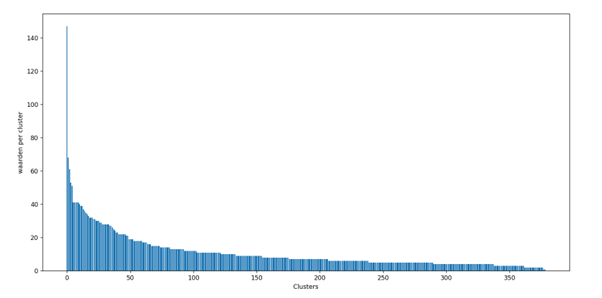
\includegraphics[width=0.7\linewidth]{../foto's/datakmeanstfidf}
    \caption{Een staafdiagram van de resultaten van tf-idf in combinatie met K-means.}
    \label{fig:staafdiagram_k-means_tf-idf}
\end{figure}



\subsection{Word2vec}
De word2vec functie wordt ingeladen met spacy. Dit verwacht een string parameter die bestaat uit vier delen, deze bepaalt welke versie van het word2vec algoritme teruggegeven wordt. Aangezien word2vec de afstand bepaalt aan de hand van de semantiek, bestaat er voor elke taal een ander algoritme natuurlijk. De parameter bestaat uit:
\\\indent
\begin{itemize}
    \item De taal: de datasets die gebruikt worden in dit onderzoek zijn in het Engels, dus wordt 'en' gebruikt. Dit kan natuurlijk ook in andere talen zoals Nederlands en Frans.
    \item Het type: 'core' is de enige mogelijkheid in het Engels.
    \item De data waarmee het algoritme getraind is: 'web' is de enige mogelijkheid in het Engels. In het Nederlands moet deze waard verplicht 'news' zijn, het Nederlandse algoritme is dus enkel getraind met data van nieuws en media.
    \item De size: de mogelijkheden zijn 'sm', 'md', 'lg' en 'trf'. Hoe smaller de size, hoe sneller en efficiënter het algoritme gebruikt kan worden, hoe groter de size, hoe accurater de resultaten zijn.
\end{itemize}
\\\indent
Word2vec gebruikt de betekenis van een woord om het daarna een vector toe te wijzen, maar als in onze data verschillende code of afmetingen staan zoals '454mm', dan kan het gebeuren dat word2vec daar niet mee overweg kan. Om die reden zijn verschillende tekens aangepast in de data. Zo zijn bijvoorbeeld alle $/$ tekens vervangen door een 9, alle $*$ tekens door een 8.
\\\indent
Vervolgens maakt numpy een lege array aan. Aan deze array wordt zijn shape meegegeven met als $x$ de shape van de originele dataset en als $y$ moet het eruitzien zoals een uitkomst van het word2vec algoritme. Dit wordt verkregen door het algoritme aan te roepen met als waarde 'test' en daarvan zijn shape te gebruiken.
\\\indent
Daarna wordt geïtereerd over alle rijen van de dataset. Voor iedere rij wordt de tekst omgezet naar een vector met behulp van het word2vec algoritme. Deze vector wordt aan de aangemaakte array op de juiste plaats toegevoegd.


\begin{lstlisting}
word2vec = spacy.load('en_core_web_md')
doc= np.empty(shape=(df_original.shape[0], word2vec("test").vector.shape[0]))

for idx, line in df_original.iterrows():
    vector = word2vec(line[chosen_column]).vector
    doc[idx] =vector


\end{lstlisting}



\subsection{Dbscan}
De DBSCAN() functie wordt net zoals K-means geïmporteerd van sklearn. Deze heeft twee parameters nodig, een eps en een minimum samples. De eps is de straal van de cirkel die rond ieder punt getrokken wordt en de minimum samples is het aantal punten er in die cirkel moeten liggen om een Core Point te worden. Om de beste waarden te vinden, werd gewerkt met een dubbele for lus zodat allerlei combinaties geprobeerd konden worden.
\\\indent
Al snel werd duidelijk dat er voor deze doelstelling slechts twee mogelijkheden zijn voor het minimum aantal samples, namelijk 1 of 2. De uitkomst is echter gelijk voor deze twee mogelijkheden. Het enige verschil is dat bij een minimum van 1 alle waarden die niet dicht bij andere waarden liggen helemaal alleen in een aparte cluster zitten en bij een minimum van twee zitten deze waarden simpelweg niet in een cluster. Het label van hun cluster staat dan op -1, dit kan op zich gezien worden als een aparte cluster waar alle restwaarden in zitten. In dit onderzoek wordt gewerkt met een minimum van 2 zodat het aantal succesvolle clusters gekend is.
\\\indent
De straal van de cirkel was iets lastiger om te bepalen. Bij het proberen van waarde 1 had één cluster 1600 waarden. Toen 1 te veel bleek, werd 0.5 geprobeerd. Dit bleek echter te weinig, want 1100 waarden van de 4000 waren niet aan een cluster toegevoegd. Als volgende werd 0.75 geprobeerd, met nog steeds meer dan 800 waarden die niet tot een cluster behoorden. De ideale waarde lag hierdoor duidelijk tussen 0.75 en 1. Er werd niet direct een perfecte waarde gevonden aangezien er nog altijd veel waarden niet aan een cluster werden toegevoegd en tegelijkertijd werd de grootste succesvolle cluster maar groter en groter. Toen werd er gezocht naar een waarde waarbij de het aantal waarden in die twee clusters ongeveer gelijk was. Uiteindelijk werd tot de conclusie gekomen dat 0.92 als beste straal aangeduid, aangezien zo'n 660 waarden niet tot een cluster behoorden en de grootste succesvolle cluster zo'n 670 waarden bevatte.
\\\indent

\begin{lstlisting}

    db = DBSCAN(eps=0.92, min_samples=2).fit(tfidf_vectorizer_vectors)

\end{lstlisting}



\subsection{Levenshtein}
Om hiërarchisch te kunnen clusteren, zijn alle afstanden nodig tussen alle waarden. Eerst wordt de dataset omgezet in een lijst. Daarna wordt een lege array aangemaakt en de lengte van de lijst wordt gebruikt als het aantal rijen en het aantal kolommen. Zo wordt het een twee-dimensionale array ook wel matrix genoemd. Ook wordt het datatype van deze array op integer gezet. Vervolgens wordt gewerkt met een dubbele for lus zodat alle combinaties tussen alle waarden overlopen worden. Voor elke combinatie wordt de distance() functie aangeroepen, deze is geïmporteerd van Levenshtein en zal de levenshtein distance tussen de twee waarden teruggeven. Deze afstand wordt dan op de juiste plaats in de matrix geplaatst.
\\\indent

\begin{lstlisting}
data_list = df_original[chosen_column].to_list()

Matrix = np.zeros((len(data_list),len(data_list)),dtype=np.int)

for i in range(0,len(data_list)):
    for j in range(0,len(data_list)):
        Matrix[i,j] = distance(data_list[i],data_list[j])

\end{lstlisting}


\subsection{Hiërarchisch clusteren}
Het hiërarchisch clusteren wordt gedaan met behulp van Scipy, dit is een wetenschappelijk rekenpakket voor Python. Van Scipy worden de functies linkage(), dendrogram() en fcluster() gebruikt. De linkage functie is de functie die clustert, hij krijgt de matrix met afstanden mee en een methode. Deze methode bepaalt hoe de afstand tussen een waarde en een cluster berekend wordt. Bij $complete$ wordt de verste afstand gebruikt, bij $single$ de kortste afstand en bij $average$ het gemiddelde van alle afstanden. Vervolgens kan een dendrogram gemaakt worden van deze data. Bij het tonen van het plot, wordt de onderstaande figuur weergegeven.
\\\indent
\begin{lstlisting}
linkage_data = linkage(Matrix, method='complete')
dendrogram(linkage_data)
plt.show()
\end{lstlisting}
\\\indent
\begin{figure}[h]
    \centering
    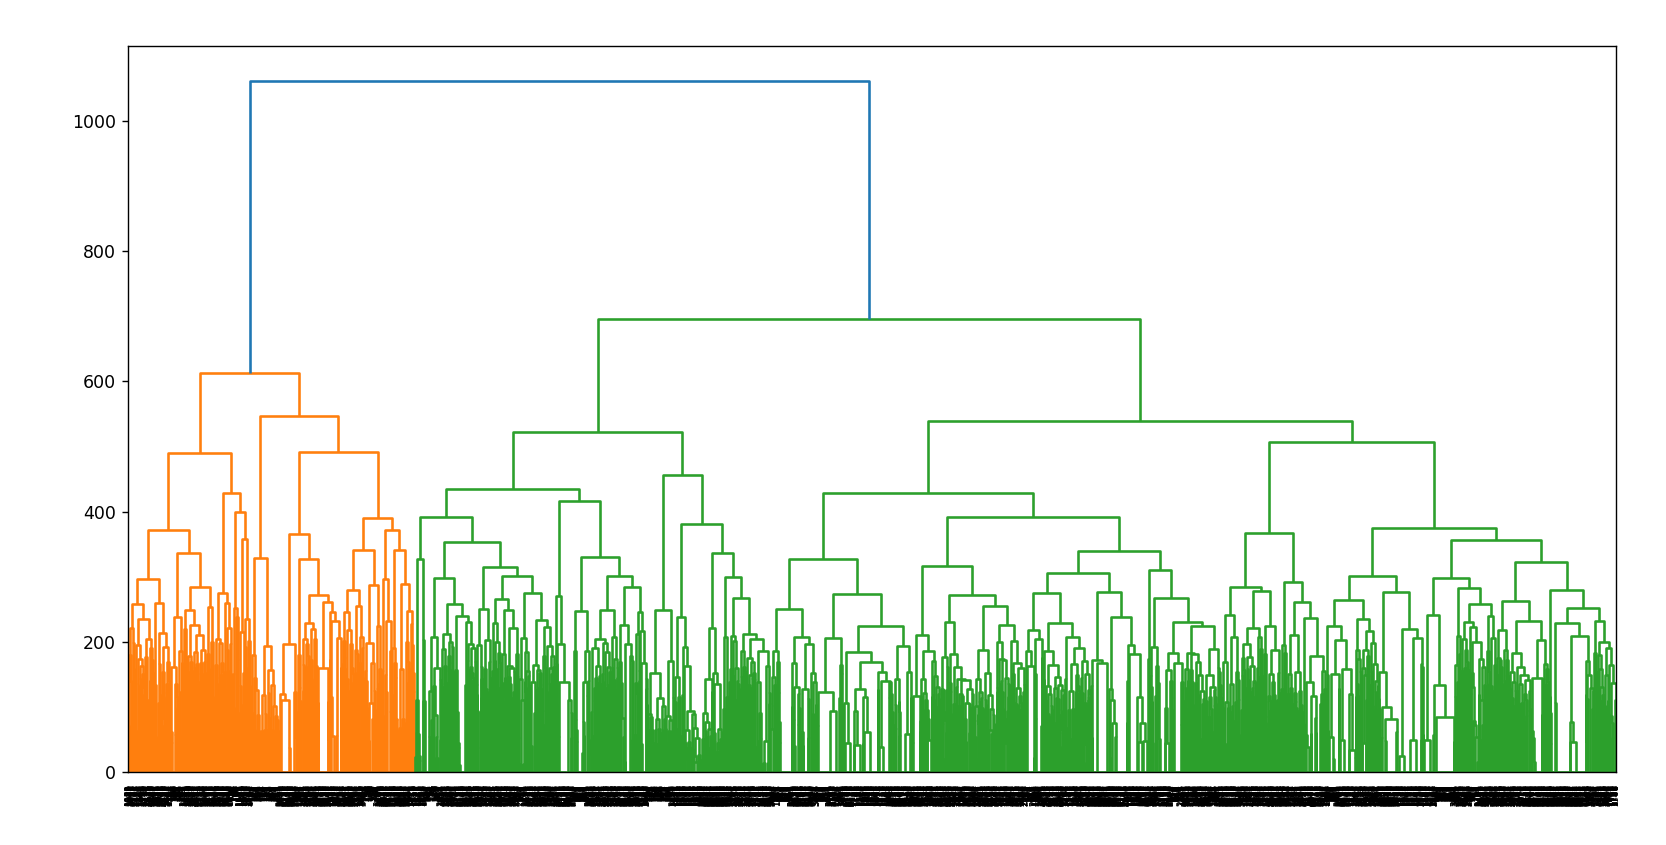
\includegraphics[width=0.7\linewidth]{../foto's/dendogram}
    \caption{Dendrogram van het hiërarchisch clusteren.}
    \label{fig:dendrogram}
\end{figure}
\\\indent
Uit het dendrogram alleen is weinig af te leiden aangezien dit blijft doorgaan totdat alle waarden in één cluster zitten. Het dendrogram moet als het ware horizontaal doorgesneden worden op de juiste plaats zodat er kan berekend worden welke waarden samen in een cluster zitten. Om dit uit te voeren wordt gebruik gemaakt van de fcluster functie. Deze functie bepaalt waar de horizontale scheiding ligt door te kijken naar de afstand tussen twee clusters die samengevoegd worden. Als deze afstand groter is dan de treshold, dan worden de clusters niet meer samengevoegd.
\\\indent

\begin{lstlisting}

threshold = 200
final_clusters = fcluster(linkage_data, threshold, criterion='distance')

\end{lstlisting}



\section{Vergelijkende studie}
In deze sectie worden de resultaten van alle algoritmes besproken. Ook worden deze resultaten vergeleken met elkaar, zodat kan achterhaald worden welke manieren het beste werken voor verschillende situaties.
\newpage
\subsubsection{Eerste dataset}
Als eerste worden de vijf mogelijkheden uitgevoerd met de dataset die uit de praktijk komt. Hierbij wordt gekeken naar de grootste cluster, aantal clusters, gemiddelde aantal waarden per cluster, een eventuele vuilniscluster en het Silhoutte gemiddelde. Dit Silhoutte gemiddelde geeft weer hoe goed elke waarde in zijn respectievelijke cluster thuishoort in vergelijking met de andere clusters. Dit is een score tussen min één en één. Hoe hoger de score, hoe beter de clusters gevormd zijn. Als laatste wordt ook een kort willekeurig stuk uit de data getoond.

\begin{enumerate}
    \item Tf-idf en K-means:
    \begin{itemize}
        \item Grootste cluster: 147
        \item Grootte vuilniscluster: 147
        \item Aantal clusters: 378
        \item Gemiddeld aantal waarden per cluster: 10,96 => quasi 11
        \item Silhoutte avg: 0.47
        \item
        110 , Perfix T.B 0.0x00
        \\\indent110 , "Perfix TB/Zn 0,0X00"
        \\\indent285 , Pin Router Head Hitachi
        \\\indent83  , PIN THREADS 00 X 000
        \\\indent83  , PIN THREADS 0 X 00
        \\\indent169 , PINCE DEMONTAGE RS-EVO
        \\\indent176 , Pipe clip CUPRA D00 (CR00)
        \\\indent73  , Pipe Clip Diameter 000  B
        \\\indent73  , Pipe Clip Diameter 000  G
        \begin{figure}[h]
            \centering
            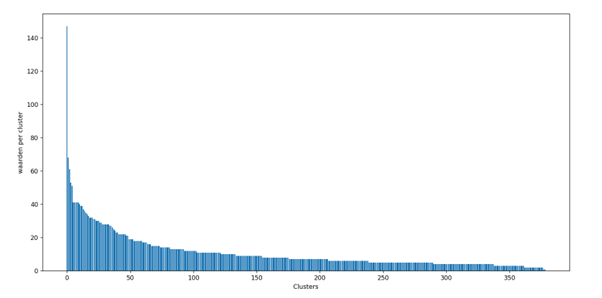
\includegraphics[width=0.7\linewidth]{../foto's/datakmeanstfidf}
            \caption{Resultaten tf-idf met K-means voor de eerste dataset}
            \label{fig:dataset1_kmeans_tfidf}
        \end{figure}
    \end{itemize}
\newpage
\item Levenshtein distance en hiërarchisch clusteren:
\begin{itemize}
    \item Grootste cluster: 67
    \item Grootte vuilniscluster: Niet gevonden
    \item Aantal clusters: 560
    \item Gemiddeld aantal waarden per cluster: 7,40
    \item Silhoutte avg: 0.44
    \item
    361 , Perfix T.B 0.0x00
    \\\indent361 , "Perfix TB/Zn 0,0X00"
    \\\indent442 , Pin Router Head Hitachi
    \\\indent377 , PIN THREADS 00 X 000
    \\\indent377 , PIN THREADS 0 X 00
    \\\indent456 , PINCE DEMONTAGE RS-EVO
    \\\indent393 , Pipe clip CUPRA D00 (CR00)
    \\\indent397 , Pipe Clip Diameter 000  B
    \\\indent397 , Pipe Clip Diameter 000  G
    \begin{figure}[h]
        \centering
        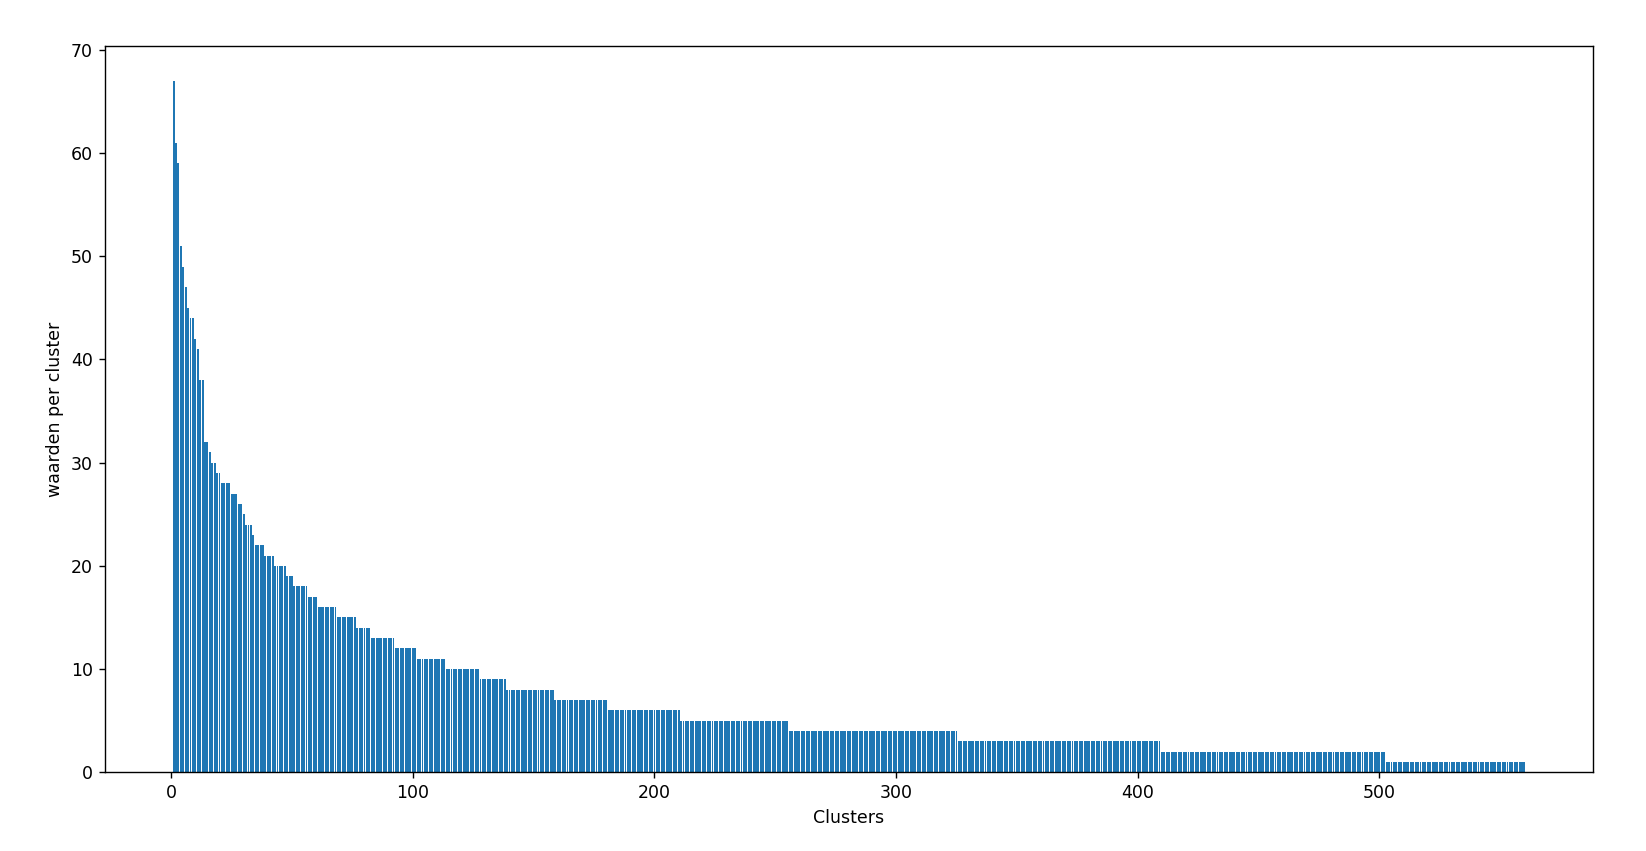
\includegraphics[width=0.7\linewidth]{../foto's/datalev}
        \caption{Resultaten hiërarchisch clusteren voor de eerste dataset}
        \label{fig:dataset1_hiërarchisch}
    \end{figure}
\end{itemize}
\newpage

\item Tf-idf en dbscan:
\begin{itemize}
    \item Grootste cluster: 577
    \item Grootte vuilniscluster: 559
    \item Aantal clusters: 384
    \item Gemiddeld aantal waarden per cluster: 10,80
    \item Silhoutte avg: 0.36
    \item
    -1 , Perfix T.B 0.0x00
    \\\indent-1 , "Perfix TB/Zn 0,0X00"
    \\\indent-1 , Pin Router Head Hitachi
    \\\indent248 , PIN THREADS 00 X 000
    \\\indent248 , PIN THREADS 0 X 00
    \\\indent-1 , PINCE DEMONTAGE RS-EVO
    \\\indent-1 , Pipe clip CUPRA D00 (CR00)
    \\\indent249 , Pipe Clip Diameter 000  B
    \\\indent249 , Pipe Clip Diameter 000  G
    \begin{figure}[h]
        \centering
        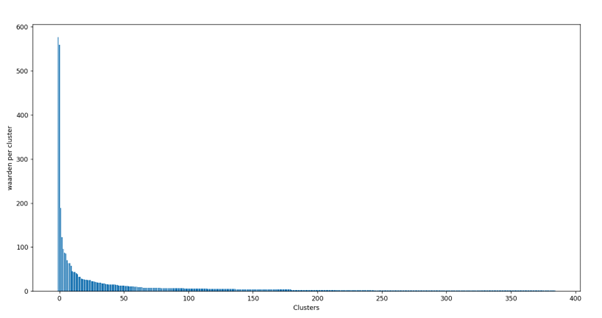
\includegraphics[width=0.7\linewidth]{../foto's/datatfidfdbscan}
        \caption{Resultaten tf-idf met dbscan voor de eerste dataset}
        \label{fig:dataset1_tf-idf_dbscan}
    \end{figure}
\end{itemize}
\newpage

\item Word2vec en K-means:
\begin{itemize}
    \item Grootste cluster: 67
    \item Grootte vuilniscluster: Niet gevonden
    \item Aantal clusters: 524
    \item Gemiddeld aantal waarden per cluster: 7,91
    \item Silhoutte avg:  0.64
    \item
    377 , Perfix T.B 0.000 0
    \\\indent443 , Perfix TB 9 Zn 0 7 000 0
    \\\indent506 , Pin Router Head Hitachi
    \\\indent415 , PIN THREADS 00 X 000
    \\\indent415 , PIN THREADS 0 X 00
    \\\indent113 , PINCE DEMONTAGE RS-EVO
    \\\indent347 , Pipe clip CUPRA D00 (C000 )
    \\\indent427 , Pipe Clip Diameter 000  B
    \\\indent384 , Pipe Clip Diameter 000  G
    \begin{figure}[h]
        \centering
        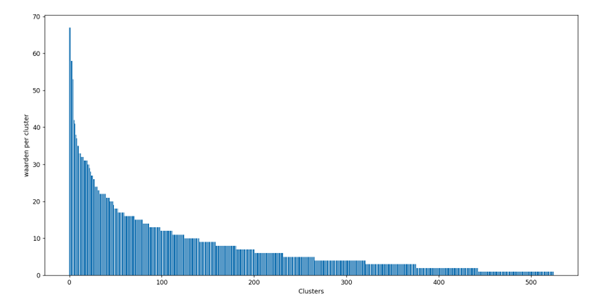
\includegraphics[width=0.7\linewidth]{../foto's/datakmeansword2vec}
        \caption{Resultaten word2vec met K-means voor de eerste dataset}
        \label{fig:dataset1_word2vec_kmeans}
    \end{figure}
\end{itemize}
\newpage

\item Word2vec en dbscan:
\begin{itemize}
    \item Grootste cluster: 785
    \item Grootte vuilniscluster: 675
    \item Aantal clusters: 332
    \item Gemiddeld aantal waarden per cluster: 12,94
    \item Silhoutte avg:  0.16
    \item
    -1 , Perfix T.B 0.000 0
    \\\indent-1 , Perfix TB 9 Zn 0 7 000 0
    \\\indent-1 , Pin Router Head Hitachi
    \\\indent-1 , PIN THREADS 00 X 000
    \\\indent-1 , PIN THREADS 0 X 00
    \\\indent66 , PINCE DEMONTAGE RS-EVO
    \\\indent216 , Pipe clip CUPRA D00 (C000 )
    \\\indent223 , Pipe Clip Diameter 000  B
    \\\indent224 , Pipe Clip Diameter 000  G
    \begin{figure}[h]
        \centering
        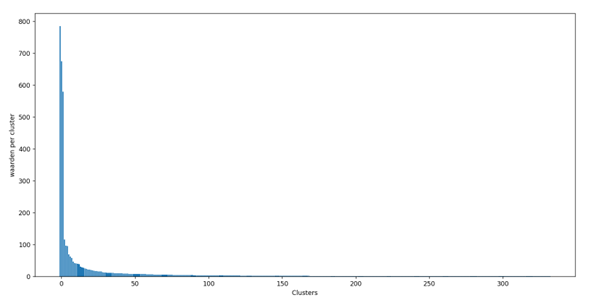
\includegraphics[width=0.7\linewidth]{../foto's/datadbscanword2vec}
        \caption{Resultaten word2vec met dbscan voor de eerste dataset}
        \label{fig:dataset1_word2vec_dbscan}
    \end{figure}
\end{itemize}
\end{enumerate}
\\\indent
Als laatste wordt de gelijkenis tussen de vijf resultaten berekend. Dit gebeurt door de adjusted\_rand\_score() functie die afkomstig is van sklearn. Deze functie vergelijkt de cluster resultaten en geeft een getal tussen nul en één terug. Hoe hoger dit getal is, hoe dichter de resultaten bij elkaar liggen.
\\\indent

\\\indent(Word2vec met Kmeans) - (Hiërarchisch):\hfill ARI = 0.51
\\\indent(Tf-idf met Kmeans) - (Hiërarchisch):\hfill ARI = 0.46
\\\indent(Tf-idf met Kmeans) - (Word2vec met Kmeans):\hfill ARI = 0.43
\\\indent(Tf-idf met dbscan) - (Word2vec met dbscan):\hfill ARI = 0.21
\\\indent(Tf-idf met Kmeans) - (Tf-idf met dbscan):\hfill ARI = 0.18
\\\indent(Hiërarchisch) - (Tf-idf met dbscan):\hfill ARI = 0.12
\\\indent(Word2vec met Kmeans) - (Tf-idf met dbscan):\hfill ARI = 0.11
\\\indent(Tf-idf met Kmeans) - (Word2vec met dbscan):\hfill ARI = 0.07
\\\indent(Word2vec met Kmeans) - (Word2vec met dbscan):\hfill ARI = 0.07
\\\indent(Hiërarchisch) - (Word2vec met dbscan):\hfill ARI = 0.06

\\\indent

De resultaten worden gerangschikt van groot naar klein en door deze scores te bekijken valt op dat er drie scores hoger zijn dan de rest. Dit zijn de combinaties tussen Kmeans en Hiërarchisch clusteren. Hieruit kan afgeleid worden dat de resultaten van het clusteren met dbscan heel verschillend zijn van de rest. Dit wil nog niet perse zeggen dat het slecht is, maar het is geen goed teken.
\\\indent
Als tweede worden de silhoutte gemiddelde's vergeleken. 0.64, 0.47, 0.44, 0.36 en 0.16. Ook hier valt op dat de gemiddelde's bij het clusteren met dbscan de slechtste resultaten weergeeft. Kmeans in combinatie met Word2vec scoort hier duidelijk het hoogst.
\\\indent
Als derde wordt de grafiek bekeken. Ook hier valt dbscan direct op. Door alle toppen van de staven te verbinden kan een variatie op de 1/x grafiek ingebeeld worden. Bij de twee dbscan grafieken valt op dat die lijn enorm snel verticaal naar beneden gaat en vervolgens nog heel lang quasi horizontaal doorgaat. Dit betekent dat er een paar clusters heel veel waarden bevatten en dat er enorm veel clusters zijn die slechts een paar waarden hebben.
\\\indent
Bij de drie andere grafieken gebeurt de overgang van verticaal naar horizontaal veel trager, wat positief is. Dit wil zeggen dat de clusters beter verdeeld zijn.
\\\indent
Wat nog opvalt bij dbscan is de hoeveelheid waarden die niet tot een cluster behoren. Het feit dat ongeveer 600 van de 4000 waarden niet aan een cluster zijn toegewezen, is zeker niet de bedoeling bij deze onderzoeksvraag.
\\\indent



\newpage

\subsubsection{Tweede dataset}
Als tweede dataset wordt de data met informatie over wijnen gebruikt. Dezelfde kenmerken worden vergeleken.
\\\indent

\begin{enumerate}
    \item Tf-idf met n-grammen op basis van karakters en K-means:
    \begin{itemize}
        \item Grootste cluster: 108
        \item Grootte vuilniscluster: Niet gevonden
        \item Aantal clusters: 111
        \item Gemiddeld aantal waarden per cluster:36,04
        \item Silhoutte avg: -0.0004
        \\\indent
        \begin{figure}[h]
            \centering
            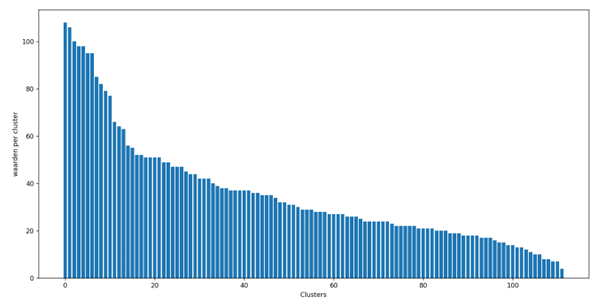
\includegraphics[width=0.7\linewidth]{../foto's/winedatatfidfkmeans}
            \caption{Resultaten tf-idf, op basis van karakters, met K-means voor de tweede dataset}
            \label{fig:dataset2_tf-idf_kmeans_char}
        \end{figure}
    \end{itemize}
    \newpage
    \item Tf-idf met n-grammen op basis van woorden en K-means:
    \begin{itemize}
        \item Grootste cluster: 35
        \item Grootte vuilniscluster: Niet gevonden
        \item Aantal clusters: 358
        \item Gemiddeld aantal waarden per cluster: 11,17
        \item Silhoutte avg: 0.0019
        \\\indent
        \begin{figure}[h]
            \centering
            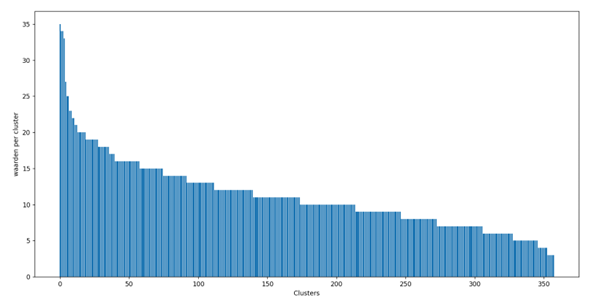
\includegraphics[width=0.7\linewidth]{../foto's/winedatatfidfkmeansword}
            \caption{Resultaten tf-idf, op basis van woorden, met K-means voor de tweede dataset}
            \label{fig:dataset2_tf-idf_kmeans_word}
        \end{figure}
    \end{itemize}
    \newpage
    \item Levenshtein distance en hiërarchisch clusteren:
    \begin{itemize}
        \item Grootste cluster: 77
        \item Grootte vuilniscluster: Niet gevonden
        \item Aantal clusters: 1146
        \item Gemiddeld aantal waarden per cluster: 3,49
        \item Silhoutte avg: 0.02
        \\\indent
        \begin{figure}[h]
            \centering
            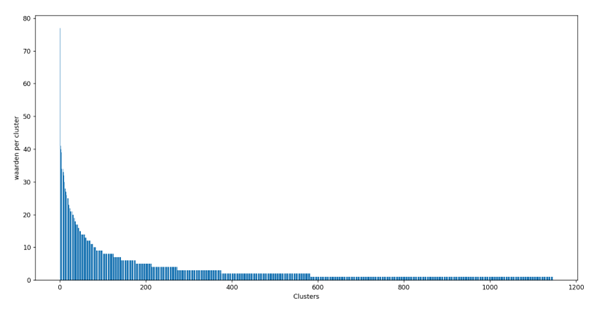
\includegraphics[width=0.7\linewidth]{../foto's/winedatalev}
            \caption{Resultaten hiërarchisch clusteren voor de tweede dataset}
            \label{fig:dataset2_hiërarchisch}
        \end{figure}
    \end{itemize}

    \newpage
    \item Tf-idf en dbscan:
    \begin{itemize}
        \item Grootste cluster: 2060
        \item Grootte vuilniscluster: 2060
        \item Aantal clusters: 261
        \item Gemiddeld aantal waarden per cluster: 15,3
        \item Silhoutte avg: 0.0017
        \\\indent
        \begin{figure}[h]
            \centering
            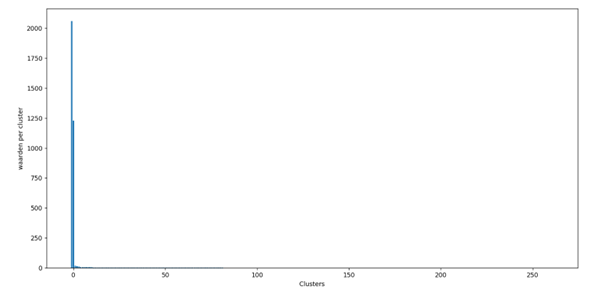
\includegraphics[width=0.7\linewidth]{../foto's/winedatatfidfdbscan}
            \caption{Resultaten tf-idf met dbscan voor de tweede dataset}
            \label{fig:dataset2_tf-idf_dbscan}
        \end{figure}
    \end{itemize}

    \newpage
    \item Word2vec en K-means:
    \begin{itemize}
        \item Grootste cluster: 18
        \item Grootte vuilniscluster: Niet gevonden
        \item Aantal clusters: 1606
        \item Gemiddeld aantal waarden per cluster: 2,49
        \item Silhoutte avg:  0.007

        \begin{figure}[h]
            \centering
            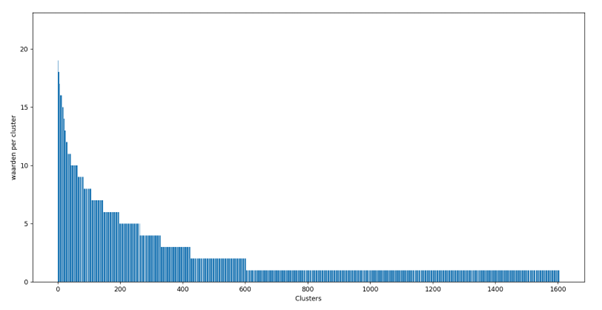
\includegraphics[width=0.7\linewidth]{../foto's/winedataword2veckmeans}
            \caption{Resultaten word2vec met K-means voor de tweede dataset}
            \label{fig:dataset2_word2vec_kmeans}
        \end{figure}
    \end{itemize}
    \newpage

    \item Word2vec en dbscan:
    \begin{itemize}
        \item Grootste cluster: 1963
        \item Grootte vuilniscluster: 1925
        \item Aantal clusters: 53
        \item Gemiddeld aantal waarden per cluster: 75,47
        \item Silhoutte avg:  -0.23

        \begin{figure}[h]
            \centering
            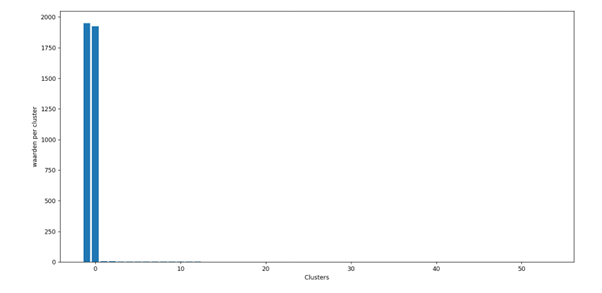
\includegraphics[width=0.7\linewidth]{../foto's/winedataword2vecdbscan}
            \caption{Resultaten word2vec met dbscan voor de tweede dataset}
            \label{fig:dataset2_word2vec_dbscan}
        \end{figure}
    \end{itemize}
\end{enumerate}

Ook voor deze dataset worden alle adjusted rand scores berekend:
\\\indent(Tf-idf, op basis van char, met Kmeans) - (Tf-idf, op basis van word, met Kmeans):\hfill ARI 0.029
\\\indent(Tf-idf met dbscan) - (Word2vec met dbscan):\hfill ARI 0.013
\\\indent(Word2vec met Kmeans) - (Tf-idf, op basis van word, met Kmeans):\hfill ARI 0.008
\\\indent(Tf-idf, op basis van word, met Kmeans) - (Hiërarchisch):\hfill ARI 0.006
\\\indent(Tf-idf, op basis van char, met Kmeans) - (Word2vec met Kmeans):\hfill ARI 0.005
\\\indent(Tf-idf, op basis van char, met Kmeans) - (Hiërarchisch):\hfill ARI 0.005
\\\indent(Tf-idf, op basis van char, met Kmeans) - (Tf-idf met dbscan):\hfill ARI 0.003
\\\indent(Word2vec met Kmeans) - (Hiërarchisch):\hfill ARI 0.003
\\\indent(Word2vec met Kmeans) - (Tf-idf met dbscan):\hfill ARI 0.0003
\\\indent(Tf-idf, op basis van char, met Kmeans) - (Word2vec met dbscan):\hfill ARI 0.002
\\\indent(Hiërarchisch) - (Tf-idf met dbscan):\hfill ARI 0.002
\\\indent(Tf-idf, op basis van word, met Kmeans) - (Tf-idf met dbscan):\hfill ARI 0.001
\\\indent(Tf-idf, op basis van word, met Kmeans) - (Word2vec met dbscan):\hfill ARI 0.001
\\\indent(Word2vec met Kmeans) - (Word2vec met dbscan):\hfill ARI 0.001
\\\indent(Hiërarchisch) - (Word2vec met dbscan):\hfill ARI 0.001
\\\indent

Uit deze scores blijkt direct dat geen van de resultaten op elkaar lijken. Ook de silhoutte gemiddelde's liggen tegen de nul en sommigen zijn zelfs negatief. Het ziet er naar uit dat geen enkele cluster methode overweg kan met data in de vorm van lange zinnen. De grafieken van Kmeans zien er op het eerste ogenblik nog wel positief uit, maar na een stuk van de geclusterde data te bekijken, lijkt dit enorm willekeurig. Zo zitten de eerste en vierde waarde die hieronder getoond worden in dezelfde cluster, terwijl dit de woorden zijn die overeenkomen in de beschrijvingen: 'aromas of', 'this tastes', 'palate', 'finish' en 'fruits'. Dit zijn niet de belangrijke woorden die voorkomen in de beschrijvingen. Er wordt te veel geclusterd op hoe de beschrijving is opgesteld in plaats van wat de beschrijving precies inhoud.
\\\indent
\\\indent 88,"Reedy green-leaning aromas of plum and raspberry feed into a creamy palate. This tastes primarily of herbal red-berry fruits that finish oaky, dry and spicy."
\\\indent 66,"This shows some pungent, boxwood-like scents up front, followed by modest passion fruit and a bit of citrus, falling away on the finish. Drink now."
\\\indent 82,"Lisboa, with its cool climate, lends itself to crisp rosés like this. This lively fruity wine is touched by hints of vanilla and layers of red-fruit flavors. It is light and ready to drink."
\\\indent 88,"Dry earthy herbal aromas of tomato, red-berry fruits and oak set up a full palate with pounding tannins. This tastes roasted and herbal, with notes of bell pepper, tomato and creamy oak. A hard-tannin finish confirms that this Merlot skipped charm school."
\\\indent 96,"This is a neutral, papery white wine, with a flat, rather than lively mouthfeel. The apple flavored fruit is there, along with a touch of licorice, but the freshness seems to have been lost along the way."
\\\indent 74,"Mula Velha, “the old donkey,” is a younger wine than its name suggests. Brisk and fruity, it offers firm tannins and layers of blackberry fruit. With a touch of oak aging, the wine is developing well and will be ready to drink from late 2017."
\\\indent 82,"This wine is ripe, full of black fruits and soft tannins. With plenty of acidity to keep it crisp, the wine has a cool, flavorful character topped off by berry fruits. It's ready to drink."
\\\indent 111,"This wine is light in tannins and ripe in fruit, with a delicious red-berry character. Drink this attractive wine from 2019."
\\\indent 111,"This is a soft, ripe and fruity wine. It has gentle tannins and attractive red-berry fruits. There is just a touch of dryness that gives this easygoing wine its structure. Drink from early 2017."


\newpage


\subsubsection{Derde dataset}
Als derde en laatste dataset wordt de data met productinformatie over retail producten gebruikt. Dezelfde kenmerken worden vergeleken.
\\\indent

\begin{enumerate}
    \item Tf-idf met n-grammen op basis van karakters en K-means:
    \begin{itemize}
        \item Grootste cluster: 108
        \item Grootte vuilniscluster: 108
        \item Aantal clusters: 583
        \item Gemiddeld aantal waarden per cluster: 8,55
        \item Silhoutte avg: 0.62
        \item 400 , BLACK CHRISTMAS TREE
        \\\indent 400 , PINK AND WHITE CHRISTMAS TREE
        \\\indent 387 , IVORY STRING CURTAIN WITH POLE
        \\\indent 18 , BLUE FELT HANGING HEART W FLOWER
        \\\indent 18 , PINK FELT HANGING HEART W FLOWER
        \\\indent 479 , SMALLFOLKART BAUBLE CHRISTMAS DEC
        \\\indent 388 , FOLKART ZINC HEART CHRISTMAS DEC
        \\\indent 388 , FOLKART CLIP ON STARS

        \begin{figure}[h]
            \centering
            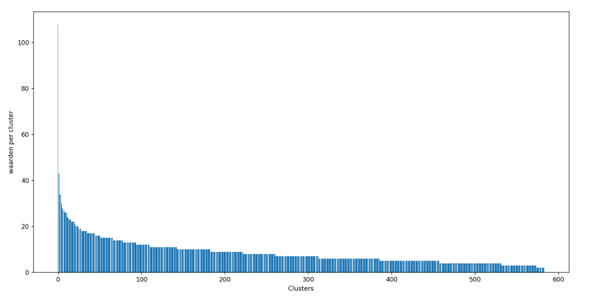
\includegraphics[width=0.7\linewidth]{../foto's/retailtfidfkmeans}
            \caption{Resultaten tf-idf, op basis van karakters, met K-means voor de derde dataset}
            \label{fig:dataset3_tf-idf_kmeans_char}
        \end{figure}
    \end{itemize}
\newpage
    \item Tf-idf met n-grammen op basis van woorden en K-means:
    \begin{itemize}
        \item Grootste cluster: 364
        \item Grootte vuilniscluster: 364
        \item Aantal clusters: 1161
        \item Gemiddeld aantal waarden per cluster: 4,30
        \item Silhoutte avg: 0.87
        \item
        773 , BLACK CHRISTMAS TREE
        \\\indent 1025 , PINK AND WHITE CHRISTMAS TREE
        \\\indent 1128 , IVORY STRING CURTAIN WITH POLE
        \\\indent 909 , BLUE FELT HANGING HEART W FLOWER
        \\\indent 909 , PINK FELT HANGING HEART W FLOWER
        \\\indent 376 , SMALLFOLKART BAUBLE CHRISTMAS DEC
        \\\indent 410 , FOLKART ZINC HEART CHRISTMAS DEC
        \\\indent 148 , FOLKART CLIP ON STARS


        \begin{figure}[h]
            \centering
            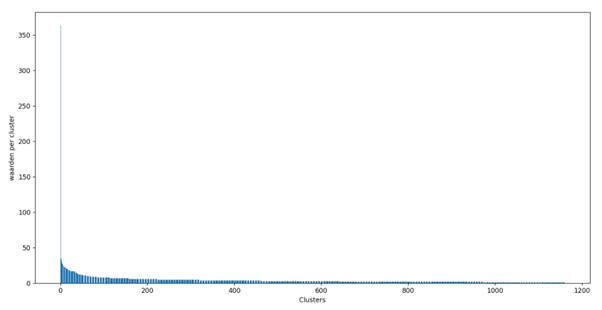
\includegraphics[width=0.7\linewidth]{../foto's/retailtfidfkmeansword}
            \caption{Resultaten tf-idf, op basis van woorden, met K-means voor de derde dataset}
            \label{fig:dataset3_tf-idf_kmeans_word}
        \end{figure}
    \end{itemize}
    \newpage
    \item Levenshtein distance en hiërarchisch clusteren:
    \begin{itemize}
        \item Grootste cluster: 263
        \item Grootte vuilniscluster: 263
        \item Aantal clusters: 174
        \item Gemiddeld aantal waarden per cluster: 28,66
        \item Silhoutte avg: 0.28
        \item 152 , BLACK CHRISTMAS TREE
        \\\indent 63 , PINK AND WHITE CHRISTMAS TREE
        \\\indent 21 , IVORY STRING CURTAIN WITH POLE
        \\\indent 21 , BLUE FELT HANGING HEART W FLOWER
        \\\indent 21 , PINK FELT HANGING HEART W FLOWER
        \\\indent 24 , SMALLFOLKART BAUBLE CHRISTMAS DEC
        \\\indent 24 , FOLKART ZINC HEART CHRISTMAS DEC
        \\\indent 80 , FOLKART CLIP ON STARS
        \begin{figure}[h]
            \centering
            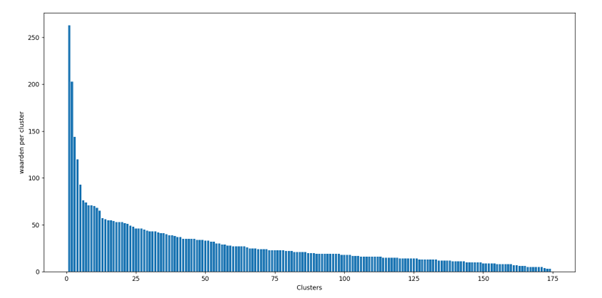
\includegraphics[width=0.7\linewidth]{../foto's/retaillev}
            \caption{Resultaten hiërarchisch clusteren voor de derde dataset}
            \label{fig:dataset3_hiërarchisch}
        \end{figure}
    \end{itemize}
    \newpage

    \item Tf-idf en dbscan:
    \begin{itemize}
        \item Grootste cluster: 333
        \item Grootte vuilniscluster: 333
        \item Aantal clusters: 673
        \item Gemiddeld aantal waarden per cluster: 7,41
        \item Silhoutte avg: 0.62
        \item
        506 , BLACK CHRISTMAS TREE
        \\\indent506 , PINK AND WHITE CHRISTMAS TREE
        \\\indent-1 , I VORY STRING CURTAIN WITH POLE
        \\\indent620 , BLUE FELT HANGING HEART W FLOWER
        \\\indent620 , PINK FELT HANGING HEART W FLOWER
        \\\indent507 , SMALLFOLKART BAUBLE CHRISTMAS DEC
        \\\indent508 , FOLKART ZINC HEART CHRISTMAS DEC
        \\\indent-1 , FOLKART CLIP ON STARS
        \begin{figure}[h]
            \centering
            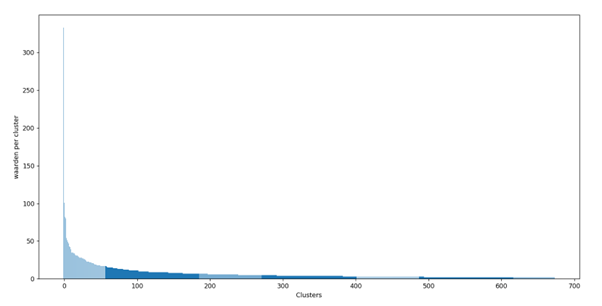
\includegraphics[width=0.7\linewidth]{../foto's/retailtfidfdbscan}
            \caption{Resultaten tf-idf met dbscan voor de derde dataset}
            \label{fig:dataset3_tf-idf_dbscan}
        \end{figure}
    \end{itemize}
    \newpage

    \item Word2vec en K-means:
    \begin{itemize}
        \item Grootste cluster: 168
        \item Grootte vuilniscluster: 168
        \item Aantal clusters: 155
        \item Gemiddeld aantal waarden per cluster: 32,17
        \item Silhoutte avg:  0.31
        \item 63 , BLACK CHRISTMAS TREE
        \\\indent 24 , PINK AND WHITE CHRISTMAS TREE
        \\\indent 84 , IVORY STRING CURTAIN WITH POLE
        \\\indent 131 , BLUE FELT HANGING HEART W FLOWER
        \\\indent 131 , PINK FELT HANGING HEART W FLOWER
        \\\indent 80 , SMALLFOLKART BAUBLE CHRISTMAS DEC
        \\\indent 80 , FOLKART ZINC HEART CHRISTMAS DEC
        \\\indent 149 , FOLKART CLIP ON STARS
        \begin{figure}[h]
            \centering
            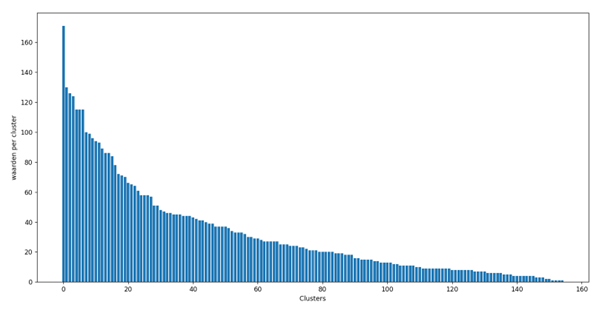
\includegraphics[width=0.7\linewidth]{../foto's/retailword2veckmeans}
            \caption{Resultaten word2vec met K-means voor de derde dataset}
            \label{fig:dataset3_word2vec_kmeans}
        \end{figure}
    \end{itemize}
    \newpage

    \item Word2vec en dbscan:
    \begin{itemize}
        \item Grootste cluster: 369
        \item Grootte vuilniscluster: 369
        \item Aantal clusters: 697
        \item Gemiddeld aantal waarden per cluster: 7,16
        \item Silhoutte avg: 0.64
        \item
        618 , BLACK CHRISTMAS TREE
        \\\indent 532 , PINK AND WHITE CHRISTMAS TREE
        \\\indent -1 , IVORY STRING CURTAIN WITH POLE
        \\\indent 655 , BLUE FELT HANGING HEART W FLOWER
        \\\indent 655 , PINK FELT HANGING HEART W FLOWER
        \\\indent 533 , SMALLFOLKART BAUBLE CHRISTMAS DEC
        \\\indent 534 , FOLKART ZINC HEART CHRISTMAS DEC
        \\\indent -1 , FOLKART CLIP ON STARS
        \begin{figure}[h]
            \centering
            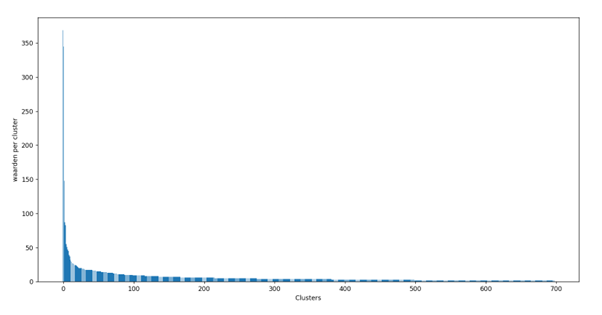
\includegraphics[width=0.7\linewidth]{../foto's/retailword2vecdbscan}
            \caption{Resultaten word2vec met dbscan voor de derde dataset}
            \label{fig:dataset3_word2vec_dbscan}
        \end{figure}
    \end{itemize}
\end{enumerate}

Ook voor de laatste dataset worden alle resultaten met elkaar vergeleken aan de hand van de adjusted rand score.

\\\indent(Tf-idf, op basis van word, met Kmeans) - (Tf-idf met dbscan):\hfill ARI =  0.44
\\\indent(Tf-idf, op basis van char, met Kmeans) - (Tf-idf met dbscan):\hfill ARI =  0.37
\\\indent(Tf-idf met dbscan) - (Word2vec met dbscan):\hfill ARI =  0.33
\\\indent(Tf-idf, op basis van word, met Kmeans) - (Word2vec met dbscan)\hfill ARI = : 0.31
\\\indent(Tf-idf, op basis van char, met Kmeans) - (Tf-idf, op basis van word, met Kmeans):\hfill ARI =  0.23
\\\indent(Word2vec met Kmeans) - (Word2vec met dbscan):\hfill ARI =  0.23
\\\indent(Tf-idf, op basis van char, met Kmeans) - (Hiërarchisch):\hfill ARI =  0.22
\\\indent(Tf-idf, op basis van char, met Kmeans) - (Word2vec met Kmeans):\hfill ARI =  0.21
\\\indent(Hiërarchisch) - (Tf-idf met dbscan):\hfill ARI =  0.21
\\\indent(Tf-idf, op basis van char, met Kmeans) - (Word2vec met dbscan):\hfill ARI =  0.19
\\\indent(Word2vec met Kmeans) - (Tf-idf met dbscan):\hfill ARI =  0.18
\\\indent(Word2vec met Kmeans) - (Hiërarchisch):\hfill ARI =  0.15
\\\indent(Tf-idf, op basis van word, met Kmeans) - (Hiërarchisch):\hfill ARI =  0.14
\\\indent(Tf-idf, op basis van word, met Kmeans) - (Word2vec met Kmeans):\hfill ARI =  0.13
\\\indent(Hiërarchisch) - (Word2vec met dbscan):\hfill ARI =  0.13
\\\indent

Deze gemiddelde's liggen gelukkig een stuk hoger dan die bij de tweede dataset. In tegenstelling tot de vorige datasets, valt er te zien dat dbscan in combinatie met tf-idf hier redelijk goed scoort. De Silhoutte gedmiddelde's zijn: 0.87, 0.64, 0.62, 0.62, 0.31 en 0.28. Dbscan presteert hier op zich wel beter, maar het feit dat meer dan 300 waarden niet aan een cluster kunnen toegevoegd worden, blijft een probleem.
\\\indent
Het valt ook op dat de tf-idf op basis van woorden het beter doet dan diegene op basis van karakters. Dit is echter bedrieglijk, want dit komt voornamelijk omdat hij 1161 clusters gebruikt. Het Silhoutte gemiddelde duidt aan of er veel waarden eerder tot een andere cluster behoren dan degene waarin ze zitten. Aangezien er 1161 clusters zijn, en er in de data redelijk wat identieke waarden zijn, bestaan veel clusters enkel uit waarden die identiek zijn. Dit betekent inderdaad dat de meest waarden in de juiste cluster zitten, maar er zouden eigenlijk meer clusters samengevoegd moeten worden die dicht bij elkaar liggen.


\section{Resultaten}
Voor data in de vorm van lange zinnen, zoals de dataset met informatie over wijnen, is er jammer genoeg geen goede clustermethode gevonden. Deze zinnen bevatten te veel woorden waar eigenlijk geen rekening mee mag gehouden worden. Woorden zoals 'Sauvignon' of 'Merlot', die toch respectievelijk 1160 en 420 keer in de dataset voorkomen, zouden als belangrijker aanschouwd moeten worden. Een goed resultaat zou bijvoorbeeld zijn als alle Merlot wijnen in dezelfde cluster zaten. Dit is echter niet geslaagd.

\\\indent

\\\indent
Data die een stuk korter is en bestaat uit een paar woorden, afmetingen en codes, zoals de dataset met productinformatie die verkregen is uit de praktijk, is een veel beter voorbeeld van hoe ongestructureerde data er meestal uitziet. Voor dit soort data zijn er wel goede methodes gevonden. Zowel Levenshtein distance in combinatie met het hiërarchisch clusteren als tf-idf in combinatie met K-means zijn twee methodes die aangeraden worden.
\\\indent
De resultaten van beide methodes zijn heel gelijkend. Bij K-means valt op dat er een stuk minder clusters zijn waardoor waarden die minder gelijkend zijn, sneller in dezelfde cluster belanden dan bij hiërarchisch. Aangezien bij hiërarchisch clusteren met Levenshtein distance gewerkt wordt, gaan waarden die hetzelfde zijn, maar met een code of afmeting die een ander aantal karakters heeft, niet meer in dezelfde cluster zitten.
\\\indent
Onderstaande waarden bijvoorbeeld. Bij hiërarchisch zitten ze in verschillende clusters, maar bij K-means behoren ze tot dezelfde cluster.
\\\indent74 , 00\/00\/000 Sinusoidal Filler Pair (Mixed)
\\\indent73 , 00\/00\/000 Sinusoidal Filler Pair WHT
\\\indent147, 00\/00\/000 Sinusoidal Filler WHT
\\\indent



\begin{enumerate}
\item K-means: Let hierbij zeker op het gebruik van tf-idf op basis van karakters, anders geeft deze methode in deze situatie heel verschillende resultaten.
\\\indent
Voordelen:
\begin{itemize}
    \item Minder clusters.
    \item Waarden moeten maar een beetje gelijkend zijn om in dezelfde cluster te komen.
\end{itemize}
\\\indent
Nadelen:
\begin{itemize}
    \item Een duidelijke vuilniscluster.
    \item Het is wat zoeken naar een goede waarde voor T2 tijdens de canopy clustering.
\end{itemize}

\item Hiërarchisch clusteren:
\\\indent
Voordelen:
\begin{itemize}
    \item Deze clustering blijft doorgaan tot er één cluster overblijft waarbij het een stuk eenvoudiger is om uit te zoeken wat de beste plaats is om een horizontale streep te trekken in het dendrogram.
    \item Waarden in dezelfde cluster zijn steeds zeer gelijkend
    \item Geen vuilniscluster: waarden die apart horen zitten apart in een cluster
\end{itemize}
\\\indent
Nadelen:
\begin{itemize}
    \item Veel clusters.
    \item Veel waarden die wel samen horen, maar niet gelijkend genoeg zijn, waardoor ze in verschillende clusters belanden.
\end{itemize}

\end{enumerate}


\\\indent

\\\indent
Als er geen codes of afmetingen in de data voorkomen, zoals in de dataset met productinformatie uit de retail, zijn er ook een paar succesvolle methodes gevonden. Dbscan was in deze situatie op zich nog bruikbaar. Het slaagde erin heel gelijkende waarden samen te clusteren, maar de andere methodes slaagden daar even goed in en deze konden zelfs minder gelijkende waarden ook in dezelfde cluster steken. Dbscan komt hierdoor uit dit onderzoek als de minst succesvolle methode om ongestructureerde masterdata te clusteren.
\\\indent
Vervolgens blijven er nog drie methodes over. Wanneer naar de resultaten gekeken wordt, zouden de $black$ $christmas$ $tree$ en de $pink$ $and$ $white$ $christmas$ $tree$ liefst in dezelfde cluster zitten. Dit is slechts in één van de drie methodes geslaagd. K-means in combinatie met tf-idf komt ook hier naar boven als de beste cluster methode. De data is goed geclusterd, de clusters zijn relatief klein, gemiddeld slechts 8.55 waarden per cluster, maar de waarden erin passen beter bij elkaar dan in de clusters van het hiërarchisch clusteren of die van K-means in combinatie met word2vec.
\\\indent
Er is ook nog steeds een vuilniscluster met 108 waarden in. Dit is jammer, maar aan de andere kant is dit waarschijnlijk wel normaal, er zijn altijd waarden die totaal verschillend zijn van al de rest. Bij de andere twee methoden bevatte de vuilniscluster 168 en 263 waarden, dit zijn er dus nog meer. Tijdens de requirements analyse werd bepaald dat de vuilniscluster maximum 10\% van alle waarden mocht bevatten, in dit geval dus maximum 500 waarden. Dit is voldaan bij alle drie deze methodes.
\\\indent



% Voeg hier je eigen hoofdstukken toe die de ``corpus'' van je bachelorproef
% vormen. De structuur en titels hangen af van je eigen onderzoek. Je kan bv.
% elke fase in je onderzoek in een apart hoofdstuk bespreken.

%\input{...}
%\input{...}
%...

%%=============================================================================
%% Conclusie
%%=============================================================================

\chapter{Conclusie}%
\label{ch:conclusie}

% TODO: Trek een duidelijke conclusie, in de vorm van een antwoord op de
% onderzoeksvra(a)g(en). Wat was jouw bijdrage aan het onderzoeksdomein en
% hoe biedt dit meerwaarde aan het vakgebied/doelgroep?
% Reflecteer kritisch over het resultaat. In Engelse teksten wordt deze sectie
% ``Discussion'' genoemd. Had je deze uitkomst verwacht? Zijn er zaken die nog
% niet duidelijk zijn?
% Heeft het onderzoek geleid tot nieuwe vragen die uitnodigen tot verder
%onderzoek?


Uit de resultaten van de vergelijkende studie kan geconcludeerd worden dat K-means op alle vlakken de beste clustermethode is voor ongestructureerde masterdata. De methode werkt door eerst de data om te zetten in vectoren aan de hand van tf-idf, hierbij worden de strings eerst in n-grammen gesplitst met een range van 2 tot 4 karakters. Vervolgens wordt een canopy clustering uitgevoerd op deze lijst van vectoren zodat er kan bepaald worden hoeveel clusters er nodig zijn. Tot slot clustert het K-means algoritme de dataset op basis van dit aantal clusters en de vectoren van tf-idf.
\\\indent

\\\indent
Uit dit onderzoek blijkt ook dat dbscan helemaal niet geschikt is om aan de hand van tf-idf of word2vec ongestructureerde masterdata te clusteren. Hiërarchisch clusteren of K-means combineren met word2vec bleek dan weer wel in staat de data succesvol te clusteren, maar toch niet zo goed als de combinatie tussen K-means en tf-idf.
\\\indent

\\\indent
Er is echter toch nog een grote vraag die overblijft, aangezien er geen manier gevonden is om ongestructureerde masterdata in de vorm van lange zinnen succesvol te clusteren. Zijn er misschien andere methodes die over het hoofd gekeken zijn? Ook is er in dit onderzoek niet dieper ingegaan op het taggen van de clusters zodat er kan geweten zijn waarom de waarden in een cluster samen horen. Dit is bij deze een uitnodiging tot verder onderzoek.



%---------- Bijlagen -----------------------------------------------------------

\appendix

\chapter{Onderzoeksvoorstel}

Het onderwerp van deze bachelorproef is gebaseerd op een onderzoeksvoorstel dat vooraf werd beoordeeld door de promotor. Dat voorstel is opgenomen in deze bijlage.

%% TODO:
\section*{Samenvatting}

Het beheren van ongestructureerde masterdata is een probleem waar veel bedrijven mee kampen. Het is heel lastig om structuur te brengen in zulke tabellen. In dit onderzoek wordt een nieuwe manier vergeleken met bestaande manieren. Door middel van clustering en tagging zal gelijkaardige data gegroepeerd worden waarna het eenvoudiger moet zijn om aan data-extractie te doen. Er zullen requirements opgesteld worden voor de algoritmes om zo te kijken welke het best geschikt is voor deze probleemstelling. Er zal vooral vergeleken worden op vlak van accuraatheid, recall, precisie en snelheid. Aan de hand van de resultaten zal er een proof-of-concept opgesteld worden om op de efficiëntste manier aan data-extractie te doen in ongestructureerde masterdata. Er wordt verwacht dat de nieuwe methode, die gebruikt maakt van clustering en tagging, als meest geschikte algoritme voor deze doelstelling uit deze studie naar voor zal komen.

% Kopieer en plak hier de samenvatting (abstract) van je onderzoeksvoorstel.

% Verwijzing naar het bestand met de inhoud van het onderzoeksvoorstel
%---------- Inleiding ---------------------------------------------------------

\section{Introductie}%
\label{sec:introductie}
Veel bedrijven hebben wat men noemt: een vuilnistabel. Dit is een tabel met ongestructureerde masterdata. Hierin staan allerlei gegevens door elkaar, waardoor het lastig wordt om iets te doen met deze data. In dit onderzoek zal er gekeken worden naar de verschillende mogelijkheden voor data-extractie te verbeteren in zo'n tabellen. Data-extractie of gegevensextractie slaat op het ophalen van relevante gegevens uit een tabel of databank.
\\\indent
In dit onderzoek zal enkel master data onderzocht worden. Master data zijn de gegevens van een bedrijf die niet transactioneel zijn. Dit betekent dat de data niet te maken heeft met transacties zoals het plaatsen van orders bijvoorbeeld. Master data zal normaal gezien nooit veranderen. Eén van de voornaamste voorbeelden hiervan zijn productgegevens: de naam, afmetingen, prijs... Deze gegevens gaan enkel aangepast worden in uitzonderlijke gevallen.
\\\indent
Er zijn twee mogelijkheden om deze data op te slaan: gestructureerd of ongestructureerd. Gestructureerde data is georganiseerd en gegroepeerd zodat alle verschillende gegevens in een aparte tabel zitten. Als dit niet het geval is en er bestaat slechts één tabel met daarin allerlei gegevens, is er sprake van ongestructureerde data. Een voorbeeld hiervan is een tabel met de naam, prijs, afmetingen, beschrijving van het product allemaal tezamen.
\\\indent
Het grote probleem met ongestructureerde master data is het feit dat het verbeteren van de datakwaliteit een stuk moeilijker wordt. Zoeken of sorteren in zo'n tabel is heel moeilijk, ook duplicaten onderscheiden is niet gemakkelijk. Daarnaast kan het soms zelfs lastig worden om de gewenste data op te halen uit zo'n tabel.
\\\indent
In dit onderzoek zullen er verschillende mogelijkheden vergeleken worden om gelijkaardige waarden uit een tabel te vinden(Fuzzymatching). Er bestaan al een heleboel technieken en metrieken hiervoor, maar wat als we de tabel eerst gaan onderverdelen in verschillende groepen (Clustering) waarbij het de bedoeling is dat elke groep iets gelijkaardigs heeft zodat er een label aan iedere groep kan gegeven worden (Tagging). De methode clustering + tagging zal worden onderzocht en vergeleken met bestaande algoritmes die gebruik maken van andere technieken.
\\\indent
Eerst en vooral zal er worden onderzocht welke algoritmes er reeds bestaan voor clustering en/of tagging in een tabel met ongestructureerde masterdata. Ook andere algoritmes voor Fuzzymatching met verschillende technieken zullen onderzocht worden. De algoritmes met betrekking tot custering en/of tagging zullen worden vergeleken met elkaar, maar ook met de algoritmes die gebruik maken van andere technieken.
\\\indent
De vergelijkende studie zal uitgevoerd worden aan de hand van aan tabel met ongestructureerde masterdata afkomstig uit een bestaand bedrijf. Met behulp van libraries in Python zal er vergeleken worden op basis van de volgende zaken: de accuraatheid, de snelheid, de precisie (Hoeveelheid van de gevonden duplicaten die correct zijn), de recall (Hoeveelheid van de aanwezige duplicaten is gevonden).

%---------- Stand van zaken ---------------------------------------------------

\section{State-of-the-art}%
\label{sec:state-of-the-art}

Twee identieke waarden in een tabel onderscheiden is natuurlijk niet zo moeilijk. Het wordt een stuk lastiger om waarden te identificeren die gelijkend zijn, en groot voorbeeld hiervan zijn typefouten. Het is wel belangrijk om een goed algoritme te kiezen, om zo weinig mogelijk, of in het beste geval geen, vals positieve uitkomsten te krijgen.
\\\indent
Een eerste mogelijkheid is om gebruik te maken van de 'Levenshtein distance'. Deze metriek bepaald de afstand tussen twee strings aan de hand van het aantal uit te voeren operaties. Deze operaties zijn: een letter toevoegen of verwijderen en een letter veranderen. Hoe meer operaties er moeten uitgevoerd worden, hoe groter de afstand tussen twee strings.
\\\indent
Een tweede metriek om de afstand te bepalen is de 'Hamming distance'. Deze metriek transformeert alle karakters in beide strings in hun binaire vorm. Bijvoorbeeld: 'a' wordt '1100001' en 'A' wordt '1000001'. De afstand tussen beide strings wordt bepaald aan de hand van het aantal verschillen in de binaire codes van de karakters. De afstand tussen 'a' en 'A' is dus 1, aangezien er slechts één binair karakter verschilt.
\\\indent
Een derde metriek heet de 'Damerau-Levenshtein distance'. Deze metriek is quasi hetzelfde als de 'Levenshtein distance', maar met de toevoeging van de transposition-operatie. Dit houdt in dat twee karakters die naast elkaar staan, gewisseld kunnen worden en de afstand slechts met één verhoogt. Zo wordt de afstand met deze metriek tussen 'over' en 'voer' één, terwijl de 'Levenshtein distance' tussen deze woorden twee zou zijn.
\\\indent
Een vierde metriek hiervoor is de 'Affine gap distance'. Hierbij wordt er rekening gehouden met afkortingen, dit komt voornamelijk voor bij namen: 'K. Dehandschutter' in plaats van 'Kobe Dehandschutter'. Met vorige metrieken zou de afstand hiertussen zeer groot zijn, aangezien er drie letters toegevoegd moeten worden, terwijl de twee strings eigenlijk heel gelijkaardig zijn. Qua scoring zijn er verschillende mogelijkheden hiervoor. Ofwel wordt voor iedere opening van een gap de afstand met drie verhoogt, en voor iedere extra toevoeging met één. Ofwel wordt er voor elk eerste karakter dat moet aangepast worden, plus één gedaan en voor elke opvolger in de gap plus een halfje.
\\\indent
Bovenstaande afstandsmetrieken zijn allemaal character-based, deze zijn handig om typefouten te ontdekken, maar als er bijvoorbeeld 'Kobe Dehandschutter' en 'Dehandschutter Kobe' wordt vergeleken, gaat de afstand heel groot zijn. Hiervoor is er een nieuwe categorie: de Token-based techniek.
\\\indent
Binnen deze techniek zijn er twee metrieken die zullen worden onderzocht. Als eerste is er een algoritme op basis van atomic strings. Dit is een reeks karakters die gesplitst wordt door interpunctie.
\\\indent



Clustering


Het K-means clustering algoritme wordt gebruikt om te clusteren in een tabel met ongestructureerde data. Dit is een incrementeel algoritme dat één cluster center tegelijk toevoegt en evenveel keer iteraties zal uitvoeren als er waarden in de tabel zitten.



%Hier beschrijf je de \emph{state-of-the-art} rondom je gekozen onderzoeksdomein, d.w.z.\ een inleidende, doorlopende tekst over het onderzoeksdomein van je bachelorproef. Je steunt daarbij heel sterk op de professionele \emph{vakliteratuur}, en niet zozeer op populariserende teksten voor een breed publiek. Wat is de huidige stand van zaken in dit domein, en wat zijn nog eventuele open vragen (die misschien de aanleiding waren tot je onderzoeksvraag!)?

%Je mag de titel van deze sectie ook aanpassen (literatuurstudie, stand van zaken, enz.). Zijn er al gelijkaardige onderzoeken gevoerd? Wat concluderen ze? Wat is het verschil met jouw onderzoek?

%Verwijs bij elke introductie van een term of bewering over het domein naar de vakliteratuur, bijvoorbeeld~\autocite{Hykes2013}! Denk zeker goed na welke werken je refereert en waarom.

%Draag zorg voor correcte literatuurverwijzingen! Een bronvermelding hoort thuis \emph{binnen} de zin waar je je op die bron baseert, dus niet er buiten! Maak meteen een verwijzing als je gebruik maakt van een bron. Doe dit dus \emph{niet} aan het einde van een lange paragraaf. Baseer nooit teveel aansluitende tekst op eenzelfde bron.
%
%Als je informatie over bronnen verzamelt in JabRef, zorg er dan voor dat alle nodige info aanwezig is om de bron terug te vinden (zoals uitvoerig besproken in de lessen Research Methods).

% Voor literatuurverwijzingen zijn er twee belangrijke commando's:
% \autocite{KEY} => (Auteur, jaartal) Gebruik dit als de naam van de auteur
%   geen onderdeel is van de zin.
% \textcite{KEY} => Auteur (jaartal)  Gebruik dit als de auteursnaam wel een
%   functie heeft in de zin (bv. ``Uit onderzoek door Doll & Hill (1954) bleek
%   ...'')

%Je mag deze sectie nog verder onderverdelen in subsecties als dit de structuur van de tekst kan verduidelijken.

%---------- Methodologie ------------------------------------------------------
\section{Methodologie}%
\label{sec:methodologie}

Het onderzoek zal uit vier verschillende fasen bestaan.
\\\indent
Vooraleer er kan begonnen worden met algoritmes runnen, moeten de requirements opgesteld worden waaraan voldaan moet worden, dit wordt dus de eerste fase. Er zal gewerkt worden met de MoSCoW methode (Must have, Should have, Could have, Won't have). Op deze manier is het duidelijk wanneer een algoritme geschikt is en wanneer niet.
\\\indent
In de tweede fase zullen alle algoritmes in de long list van gevonden mogelijkheden voor fuzzymatching uitgeprobeerd worden op de gekregen dataset. Zo zal er al een eerste onderscheiding gemaakt kunnen worden tussen degene die geschikt zijn en degene die niet geschikt zijn. Deze afmeting gebeurt aan de hand van de opgestelde requirements. Vervolgens wordt kort gekeken waarom de gefaalde algoritmes niet geschikt zijn voor deze probleemstelling, was dit verwacht of totaal niet?
\\\indent
Hierna komt de derde fase en nu zullen de algoritmes uit de short list van geschikt algoritmes vergeleken. Eerst en vooral wordt er gekeken naar de accuraatheid. Dit wordt berekent door het aantal correcte uitkomsten te delen door het totaal aantal uitkomsten. Dit is één van de belangrijkste eigenschappen van een algoritme, aangezien de resultaten toch correct moeten zijn. Vervolgens worden de precisie en recall vergeleken aangezien deze op een gelijkaardige manier te berekenen zijn. Het is natuurlijk ook belangrijk dat het runnen van een algoritme niet te lang duurt, een volgende eigenschap die zal worden vergeleken is de snelheid van het algoritme.
\\\indent
In de vierde en laatste fase zal er een proof-of-concept worden opgesteld voor deze probleemstelling. Het algoritme dat in de vorige fase als meest geschikt naar voor kwam, zal worden gebruikt om aan te tonen of het probleem wel of niet oplosbaar is.






%Hier beschrijf je hoe je van plan bent het onderzoek te voeren. Welke onderzoekstechniek ga je toepassen om elk van je onderzoeksvragen te beantwoorden? Gebruik je hiervoor literatuurstudie, interviews met belanghebbenden (bv.~voor requirements-analyse), experimenten, simulaties, vergelijkende studie, risico-analyse, PoC, \ldots?
%
%Valt je onderwerp onder één van de typische soorten bachelorproeven die besproken zijn in de lessen Research Methods (bv.\ vergelijkende studie of risico-analyse)? Zorg er dan ook voor dat we duidelijk de verschillende stappen terug vinden die we verwachten in dit soort onderzoek!
%
%Vermijd onderzoekstechnieken die geen objectieve, meetbare resultaten kunnen opleveren. Enquêtes, bijvoorbeeld, zijn voor een bachelorproef informatica meestal \textbf{niet geschikt}. De antwoorden zijn eerder meningen dan feiten en in de praktijk blijkt het ook bijzonder moeilijk om voldoende respondenten te vinden. Studenten die een enquête willen voeren, hebben meestal ook geen goede definitie van de populatie, waardoor ook niet kan aangetoond worden dat eventuele resultaten representatief zijn.
%
%Uit dit onderdeel moet duidelijk naar voor komen dat je bachelorproef ook technisch voldoen\-de diepgang zal bevatten. Het zou niet kloppen als een bachelorproef informatica ook door bv.\ een student marketing zou kunnen uitgevoerd worden.
%
%Je beschrijft ook al welke tools (hardware, software, diensten, \ldots) je denkt hiervoor te gebruiken of te ontwikkelen.
%
%Probeer ook een tijdschatting te maken. Hoe lang zal je met elke fase van je onderzoek bezig zijn en wat zijn de concrete \emph{deliverables} in elke fase?

%---------- Verwachte resultaten ----------------------------------------------
\section{Verwacht resultaat, conclusie}%
\label{sec:verwachte_resultaten}

Er wordt verwacht dat het beste algoritme voor deze probleemstelling K-means wordt. Dit zal de tabel eerst clusteren waarna er via tagging gezocht kan worden naar duplicaten. Door het feit dat de tabel geclusterd wordt, wordt verwacht dat het algoritme sneller gerund kan worden dan anderen en dat het ook correcter kan uitgevoerd worden.



%Hier beschrijf je welke resultaten je verwacht. Als je metingen en simulaties uitvoert, kan je hier al mock-ups maken van de grafieken samen met de verwachte conclusies. Benoem zeker al je assen en de onderdelen van de grafiek die je gaat gebruiken. Dit zorgt ervoor dat je concreet weet welk soort data je moet verzamelen en hoe je die moet meten.
%
%Wat heeft de doelgroep van je onderzoek aan het resultaat? Op welke manier zorgt jouw bachelorproef voor een meerwaarde?
%
%Hier beschrijf je wat je verwacht uit je onderzoek, met de motivatie waarom. Het is \textbf{niet} erg indien uit je onderzoek andere resultaten en conclusies vloeien dan dat je hier beschrijft: het is dan juist interessant om te onderzoeken waarom jouw hypothesen niet overeenkomen met de resultaten.



%%---------- Andere bijlagen --------------------------------------------------
% TODO: Voeg hier eventuele andere bijlagen toe. Bv. als je deze BP voor de
% tweede keer indient, een overzicht van de verbeteringen t.o.v. het origineel.
%\input{...}

%%---------- Backmatter, referentielijst ---------------------------------------

\backmatter{}

\setlength\bibitemsep{2pt} %% Add Some space between the bibliograpy entries
\printbibliography[heading=bibintoc]

\end{document}
